%% !TeX program = xelatex
%% 山东科技大学硕士学位论文开题报告及论文工作计划
\documentclass[UTF8,a4paper,zihao=-4,fontset=windows]{ctexart}

\usepackage{geometry}
\geometry{a4paper, left=33.9mm, right=33.9mm, top=25.4mm, bottom=25.4mm}
\usepackage{graphicx}
\graphicspath{{figs/}}
\usepackage{booktabs}
\usepackage{array}
\usepackage{tabularx}
\usepackage{multirow}
\usepackage{float}
\usepackage{enumitem}
\usepackage{caption}
\usepackage{indentfirst}
\usepackage{xcolor}
\usepackage{newunicodechar}
\newunicodechar{ω}{\ensuremath{\omega}}
\newunicodechar{′}{\ensuremath{\prime}}
\usepackage[hidelinks,bookmarks=true]{hyperref}
\emergencystretch=1.5em

\linespread{1.5}
\setlength{\parindent}{2em}
\setlength{\parskip}{0pt}

\captionsetup{font=small, labelsep=quad, justification=centering}
\captionsetup[table]{position=top, skip=4pt}
\captionsetup[figure]{skip=6pt}

\setcounter{secnumdepth}{0}

\ctexset{
  section    = {format = {\zihao{4}\bfseries\raggedright},
                beforeskip = 1.4ex plus .3ex minus .2ex,
                afterskip  = 0.9ex},
  subsection = {format = {\zihao{-4}\bfseries\raggedright},
                beforeskip = 1.0ex plus .2ex, afterskip = 0.6ex},
  subsubsection = {format = {\zihao{-4}\bfseries\raggedright},
                beforeskip = 0.8ex plus .2ex, afterskip = 0.4ex},
}

\newcommand{\hthree}[1]{\par\vspace{0.8ex}\noindent{\bfseries #1}\par\vspace{0.4ex}}

\begin{document}
\pagestyle{plain}

%% ============ 封面 ============
\begin{titlepage}
\centering
\vspace*{1.6cm}
{\zihao{1}\bfseries 山东科技大学}\\[1.4cm]
{\zihao{2} 硕士研究生学位论文开题报告}\\[0.5cm]
{\zihao{2} 及论文工作计划}\\[2.2cm]
\begin{center}
\renewcommand{\arraystretch}{1.9}
\begin{tabular}{|p{3.4cm}|p{9.2cm}|}
\hline
论文题目 & 基于反射式 TDLAS 与多参数同步测量的横向射流火焰传递特性及主动控制实验研究 \\ \hline
研究生姓名 & 赵殿虎 \\ \hline
学号 & 202583050198 \\ \hline
导师姓名、职称 & 刘训臣\quad 教授 \\ \hline
学科、专业 & 机械 \\ \hline
研究方向 & 激光诊断 \\ \hline
入学年月 & 2025 年 9 月 \\ \hline
所属学院 & 机械电子工程学院 \\ \hline
开题时间 & 2026 年 10 月 \\ \hline
\end{tabular}
\end{center}
\vfill
{\zihao{4} 山东科技大学学位评定委员会办公室制表}\\[0.6cm]
\end{titlepage}

\section{一、立论依据}
\subsection{1、课题来源、选题依据和立论背景}
\subsubsection{（1）课题来源、选题依据和立论背景}
本课题来源于课题组在研的两个实验研究项目：横向射流火焰（jet in crossflow，JICF）熄火主动控制与反射式可调谐二极管激光吸收光谱（tunable diode laser absorption spectroscopy，TDLAS）测量方法研究。两个项目共用同一套横流燃烧试验平台，前者面向燃烧不稳定性机理与熄火主动控制，后者面向反射式激光吸收光谱与自发光高速摄影的融合定量测量，二者在研究对象、测量手段与数据需求上高度互补，具备整合为一篇学位论文的条件。

横向射流火焰广泛存在于航空发动机主燃烧室、加力燃烧室、地面燃气轮机与工业锅炉等实际燃烧装置中。横流来流与横向燃料射流之间存在强剪切相互作用，形成剪切层涡、反向旋转涡对（counter-rotating vortex pair，CVP）、尾迹涡与马蹄涡等复杂涡系结构，并伴随射流轨迹弯曲与回流区形成[1]。Mahesh 从射流与横流相互作用机制出发给出了统一的描述框架[2]；Zhang 与 Yang 分别针对稳态与振荡横流条件下的横向射流开展了数值研究，揭示了来流脉动对射流穿透深度与混合过程的影响规律[3-4]。Crabb 等早期采用热线风速仪系统测量了垂直横流射流的近场速度场，为横流射流流动结构的定量认识奠定了基础[5]；Harris 等通过可控涡生成研究了横向射流中涡结构与掺混过程的相互作用[6]；Li 等针对圆形横向燃料射流在横流中的燃烧特性开展了系统的实验研究[7]。上述流动特征决定了横流火焰对来流脉动与声学扰动高度敏感：O'Connor 通过实验可视化发现，外部声学强迫会显著改变内外剪切层的涡结构与火焰稳定位置[8]；Genova 等在高压轴向分级燃烧室中进一步考察了预热与预混程度对横流射流火焰 NOx 排放的影响[9]。当燃烧室运行接近贫油熄火边界时，火焰位置与热释放率出现大幅波动，极易诱发振荡燃烧乃至熄火，严重威胁燃烧装置的安全性与可靠性[10]。

在燃烧诊断方面，可调谐二极管激光吸收光谱技术利用气体分子对特定波长激光的选择性吸收，通过扫描吸收线型反演路径平均温度与组分柱浓度，具有非侵入、响应快、物种选择性好、定量精度高等优点，已成为燃烧场定量测量的重要手段[11-13]。Hanson 系统总结了定量激光传感器在化学动力学、推进与能源系统中的应用[11]；Goldenstein 等系统梳理了红外激光吸收光谱传感的理论基础与工程实现[12]；Allen 则对二极管激光吸收传感器在气动与燃烧流场测量中的应用进行了评述[13]。在此基础上，TDLAS 正由单点/单线测量向高速、二维定量方向发展：Liu 等采用中红外直接吸收光谱实现了声激励旋流火焰时间分辨二维温度场测量[14]；Sanders 等发展了可反演视线方向温度分布的二极管激光吸收传感器[15]；Ma 等提出基于高光谱吸收光谱的层析成像方法，实现了温度与组分浓度的二维重建[16]。近年来层析反演算法不断改进：Liu 等提出基于非结构网格的激光吸收层析重建方法，改善了有限视角下的重建精度[17]；Zhao 等研制了兼顾稳定性与空间分辨率的激光吸收光谱层析传感器并用于复杂火焰诊断[18]；Yang 等基于紫外宽带吸收层析实现了轴对称火焰温度与 OH 浓度的二维定量重建[19]。

然而，上述测量多依赖对穿式光路或多角度投影，对试验台光学通道与布置空间要求较高，在空间受限的横流燃烧平台上实施困难。将发射与接收单元集成于同侧、仅需单侧光学通道的反射式/多光程光路，是降低平台改造难度、拓展 TDLAS 适用范围的重要途径。多光程池（multipass cell）通过在有限空间内多次折返激光以延长有效吸收光程、提高探测灵敏度，其典型结构包括 White 池、Herriott 池与密集光斑（dense-pattern）结构等[20]；Kasyutich 与 Martin 采用两面柱面镜构建多光程池并用于可调谐二极管激光吸收光谱测量[21]；Zhang 等提出了可变光程多光程池的设计方法，使有效光程可按需调节[22]；Fendt 等在快速压缩膨胀机上采用 Herriott 池增强的单模光纤耦合超连续谱吸收光谱系统，实现了多参数同步燃烧诊断[23]。上述工作表明多光程/腔增强光路已具备工程可行性，但将其与自发光高速摄影进行同步、同光路融合，并用于横流火焰定量诊断的系统性研究仍较为缺乏。

本课题组已在反射式 TDLAS 与 PIV/PLIF 同时拍摄装置方面提交发明专利申请[29]，具备开展融合测量的技术积累。

在燃烧控制方面，火焰传递函数刻画了火焰热释放率对来流速度脉动的频域响应，是低阶热声网络模型的关键输入，也是预测与抑制燃烧不稳定性的核心物理模型[30]。Schuller 等建立了层流火焰传递函数的统一预测模型，给出了锥形火焰与 V 形火焰增益与相位随频率变化的解析表达[31]；Candel 等分别从燃烧动力学与控制、旋流火焰动力学等角度进行了系统综述[32-34]；Palies 等进一步发展了旋流器与湍流预混旋流火焰的联合动力学模型[35-36]；Bailly 等对火焰传递函数与描述函数理论作了专门评述[37]；Wang 等将二维波基低阶网络模型用于环形燃烧室极限环预测与声耗散率量化[38]；Poinsot[39]、Lieuwen[40]与 Dowling 等[41]分别从工程预测、非定常燃烧室物理与燃烧噪声角度给出了系统性框架。需要指出的是，上述传递函数均建立在小扰动线性假设之上；当扰动幅值增大时，火焰增益出现饱和、相位发生畸变，火焰卷曲、褶皱乃至夹断等非线性行为凸显，需采用火焰描述函数（flame describing function，FDF）刻画，并耦合燃烧室声学模型预测极限环[42]。

在测量方法上，Dharmaputra 等采用多麦克风、OH* 成像、TDLAS 与延迟时间分布模型等多手段同步测量级联燃烧室 FTF，展示了多方法交叉验证的价值[43]；国内学者亦对氢混燃料旋流预混火焰传递函数开展了实验研究[44]，并对燃气燃烧热声不稳定性的机理、表征与抑制方法进行了系统梳理[45]。然而，现有 FTF 研究多集中于旋流火焰，针对横向射流火焰的传递函数系统测量尚不多见：Choi 等虽研究了受热横流中反应横向射流对谐波速度扰动的强迫响应，但尚未建立完整的火焰传递函数[46]。在速度脉动测量方面，热线风速仪、激光多普勒测速与双麦克风声学反演是三类主流手段，其时空分辨率与适用工况各有差异[47]；传统多麦克风法依赖声学反演，存在一定的间接性与假设依赖性。

贫油熄火是限制燃烧室低排放运行的主要障碍，主动控制是拓宽稳定运行边界的有效途径。McManus 等最早系统评述了燃烧不稳定性的主动控制方法，奠定了开环与闭环控制的分类框架[48]；Docquier 等对燃烧控制与传感技术进行了系统综述[49]。在熄火前兆判别方面，Nair 与 Lieuwen 研究了预混火焰熄火过程中的声学特征[50]，Yi 与 Gutmark 提出了基于压力与化学发光信号统计特征的贫油熄火实时预测方法[51]；Zhang 等进一步利用火焰图像形态特征实现了旋流火焰贫油熄火的预测[52]；Muruganandam 等提出了基于化学发光与声学信号特征的贫油熄火主动控制方法[53]。最具代表性的是 Li 等利用可调谐二极管激光温度传感器提出 FFT\%[0-50] 熄火前兆指标，在旋流稳定燃烧器上实现了主动贫油熄火闭环控制，证明了 TDLAS 传感器用于燃烧主动控制的可行性[54]。在热声不稳定性抑制方面，开环声学强迫因无需反馈传感器、系统结构简单而受到关注：Lei 等在贫预混湍流旋流火焰上把开环强迫的作用机制拆解为“自然模式抑制”与“强迫模式放大”两个并发过程，并提出了通过双频火焰响应测量先验确定有效强迫频段的控制设计框架[55]；Liao 等首次在贫预混富氢燃烧器上实验验证了开环声学强迫抑制热声振荡的有效性，指出氢体积分数 40\% 是从放大转为抑制的关键阈值[56]；Zhao 等将研究拓展至相互耦合的双振荡器系统，表明双强迫优于单强迫、且对称双强迫的能量利用效率最高[57]。

在全球“双碳”目标推进与能源结构转型的背景下，燃气轮机正加速向贫预混、掺氢/富氢燃烧方向发展，燃烧室运行当量比不断逼近贫油熄火边界，燃烧不稳定性与熄火风险显著上升。横向射流火焰在来流脉动与声激励下的传递特性及其主动控制尚缺乏系统研究，是本课题的切入点。

\subsection{2、课题研究目的、理论意义和实际应用价值}
\subsubsection{（1）课题研究目的}
针对当前横向射流火焰研究多集中于流动与混合过程、缺乏热释放率脉动的定量表征与频域传递特性的系统测量、且主动控制手段尚未在横流火焰上验证的问题，本课题拟开展以下四方面工作：

1）建立反射式 TDLAS 与自发光高速摄影同步、同光路融合测量方法。设计并搭建仅需单侧光学通道的反射式 TDLAS 光路，以 TDLAS 定量反演的温度与 H\textsubscript{2}O 柱浓度为基准，建立自发光图像强度与热化学参数之间的定量映射关系，从而在空间受限的横流燃烧平台上同时获得“定量精度”与“二维结构分辨”，解决传统对穿式光路难以布置、自发光成像难以定量的双重难题。

2）系统测量横向射流火焰的火焰传递函数。研制课题组自研恒温式热线风速仪（constant temperature anemometry，CTA）并完成静态标定，以直接测量法获取速度脉动、并与传统多麦克风声学反演结果相互对照；结合 SiPM 热释放率脉动测量与压力脉动测量，在扫频声激励条件下提取横流火焰的 FTF 增益与相位，并通过多方法交叉验证提高结果的可信度，为横流火焰动力学响应补充实验数据。

3）构建基于 TDLAS 温度脉动指标的熄火主动控制实验系统。将 FFT\%[0-50] 熄火前兆指标由旋流火焰迁移至横向射流火焰，利用 2 $\mu$m TDLAS 测得的 H\textsubscript{2}O 吸收线温度波动构建熄火前兆判据，设计以声激励或流量调节为执行手段的闭环实验回路，验证其对火焰位置与燃烧稳定性的调控效果。

4）组织横流火焰自激热声振荡并判别主导耦合量。在贫预混条件下调整出口收缩段与带孔板孔径，使声波在上下游之间形成较强反射，诱导横流火焰产生自激热声振荡；测量其共振频率与声学模态，结合相位平均图像判别主导耦合量（火焰面积、火焰高度或当量比脉动），为传递函数测量提供与自激工况一致的物理参照。

\subsubsection{（2）理论意义}
其一，在方法层面，本课题将多光程/腔增强光路思想与自发光成像相结合，提出并验证“同光路、同步”的融合测量范式，为单侧光学接入条件下的燃烧场定量诊断提供新途径，可丰富激光吸收光谱与自发辐射诊断融合的方法学体系[23-24,29]。

其二，在物理层面，本课题拟系统测量横向射流火焰的火焰传递函数，尝试获得横流火焰增益与相位随激励频率的变化规律，并与旋流火焰、锥形/V 形层流火焰的既有结果进行对比[31,43,46]，以期为厘清剪切层涡结构演化与热释放率脉动之间的相位关系提供实验依据，补充横流火焰动力学响应数据。

其三，在控制层面，本课题把基于激光吸收光谱温度脉动的熄火前兆判别方法由旋流稳定火焰拓展至横向射流火焰，检验该类前兆指标的工况适应性与可迁移性，为贫油熄火主动控制理论提供新的实验证据[51-52,54]。

\subsubsection{（3）实际应用价值}
在航空发动机与地面燃气轮机领域，燃烧室普遍面临贫油熄火与热声振荡的双重约束。本课题拟建立的横流火焰 FTF 测量方法与熄火前兆指标，可为燃烧室稳定性预测模型的参数标定与主动控制策略开发提供实验参考，有望为拓宽低排放运行边界、提升运行安全裕度提供基础数据支持。

在测量装备层面，反射式 TDLAS 光路仅需单侧光学通道，有助于降低试验台改造的要求，配合课题组自研的低成本恒温式热线风速仪与 SiPM 探测模块，可为同类受限空间燃烧装置的诊断提供一种可借鉴的多参数同步测量方案[15,20-21]。

\section{二、文献综述}
\subsection{1、国内外研究现状、发展动态}
\subsubsection{（一）横向射流火焰流动与燃烧特性}
横向射流的流动结构研究始于 20 世纪 60—70 年代，其核心科学问题是射流与横流之间的强剪切相互作用如何决定涡系演化与掺混过程。Karagozian 在其标志性综述中系统归纳了横向射流的流场结构，指出沿射流轨迹自上游向下游依次存在剪切层涡、反向旋转涡对（CVP）、尾迹涡与马蹄涡四类典型涡结构，并进一步梳理了通过主动与被动方式控制射流轨迹与掺混的方法[1]；Mahesh 从动量比、速度比与雷诺数等无量纲参数出发，给出了射流与横流相互作用机制的统一描述框架，明确了射流轨迹弯曲、涡环卷吸与回流区形成的参数依赖关系[2]。图 1 给出了横流射流中的典型涡系结构与坐标定义。

\begin{figure}[H]
\centering
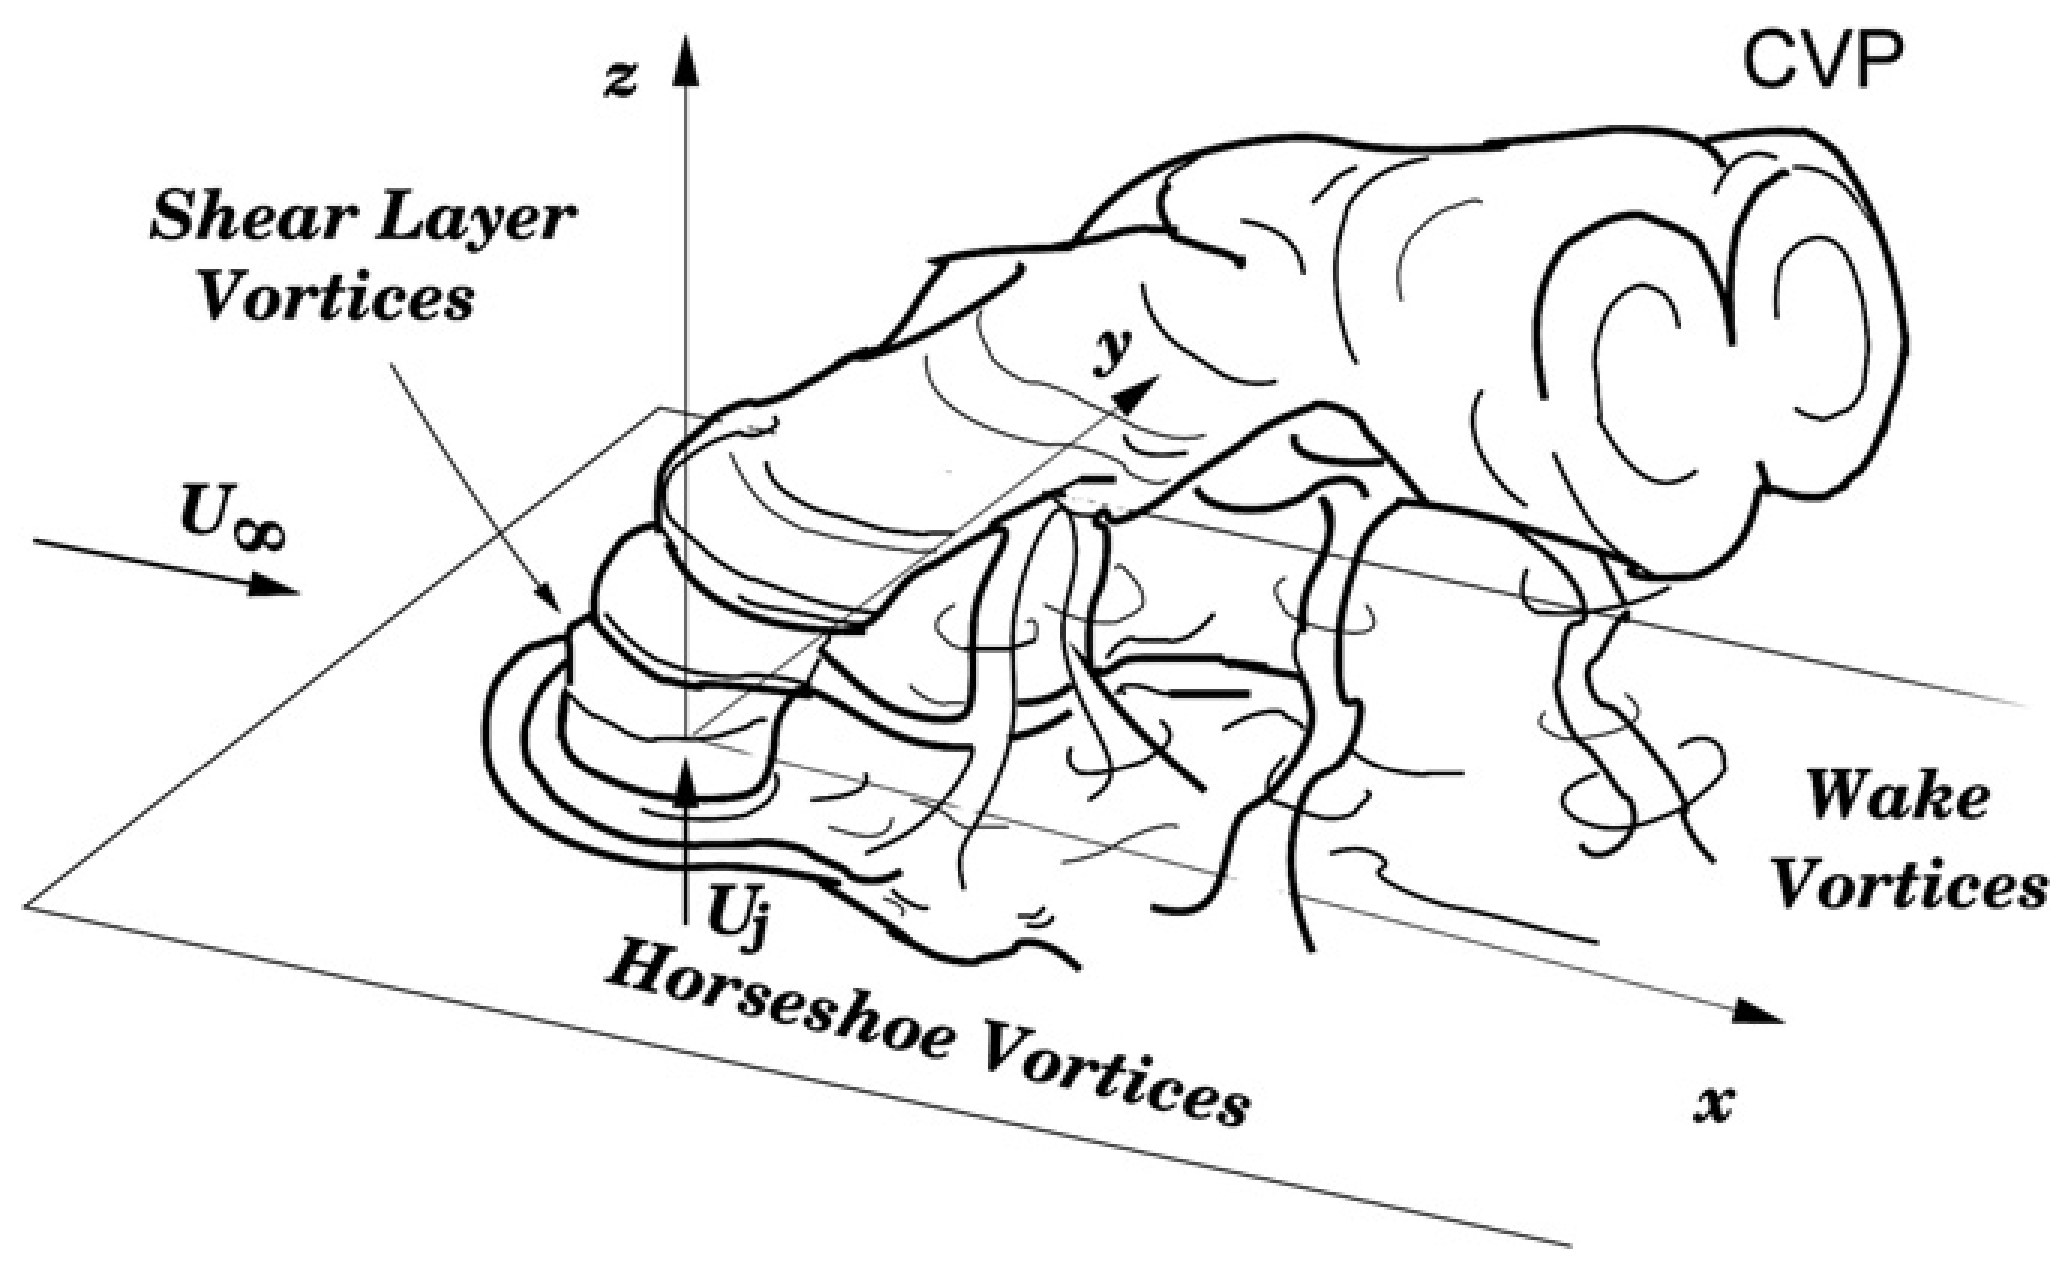
\includegraphics[width=1.000\linewidth]{figs/fig01.png}
\caption{横流射流中的涡系结构与坐标定义（引自文献[1]）}
\end{figure}
在定量流动测量方面，Crabb 等采用热线风速仪系统测量了垂直横流射流的近场速度场，获得了射流轨迹与回流区的定量数据，成为后续数值验证的经典基准[5]；Harris 等通过受控涡生成装置考察了横向射流中涡结构与掺混的相互作用，表明上游涡结构的受控引入可显著改变射流下游的混合特性[6]。在数值研究方面，Zhang 与 Yang 分别针对稳态横流与振荡横流两种工况开展了系统的大涡模拟，指出横流振荡会在剪切层中引入额外的涡卷吸过程，从而改变射流穿透深度与混合效率[3-4]。

在反应流方面，Li 等针对圆形横向燃料射流在横流中的燃烧特性开展了系统实验，考察了动量比与当量比对火焰形态、火焰长度与燃烧效率的影响[7]；Genova 等在高压轴向分级燃烧室中研究了预热与预混程度对横流射流火焰 NOx 排放的影响，指出预热会缩短点火延迟并改变射流火焰的稳定位置[9]。在声学强迫响应方面，O'Connor 通过实验可视化研究了横向强迫作用下剪切层动力学与火焰响应，结果表明外部声学强迫会显著改变内外剪切层的涡结构与火焰稳定位置，声强迫幅值与频率共同决定火焰形态的响应模式[8]。图 2 给出了横向声强迫下内剪切层涡形成事件与火焰褶皱演化的典型图像[8]。

\begin{figure}[H]
\centering
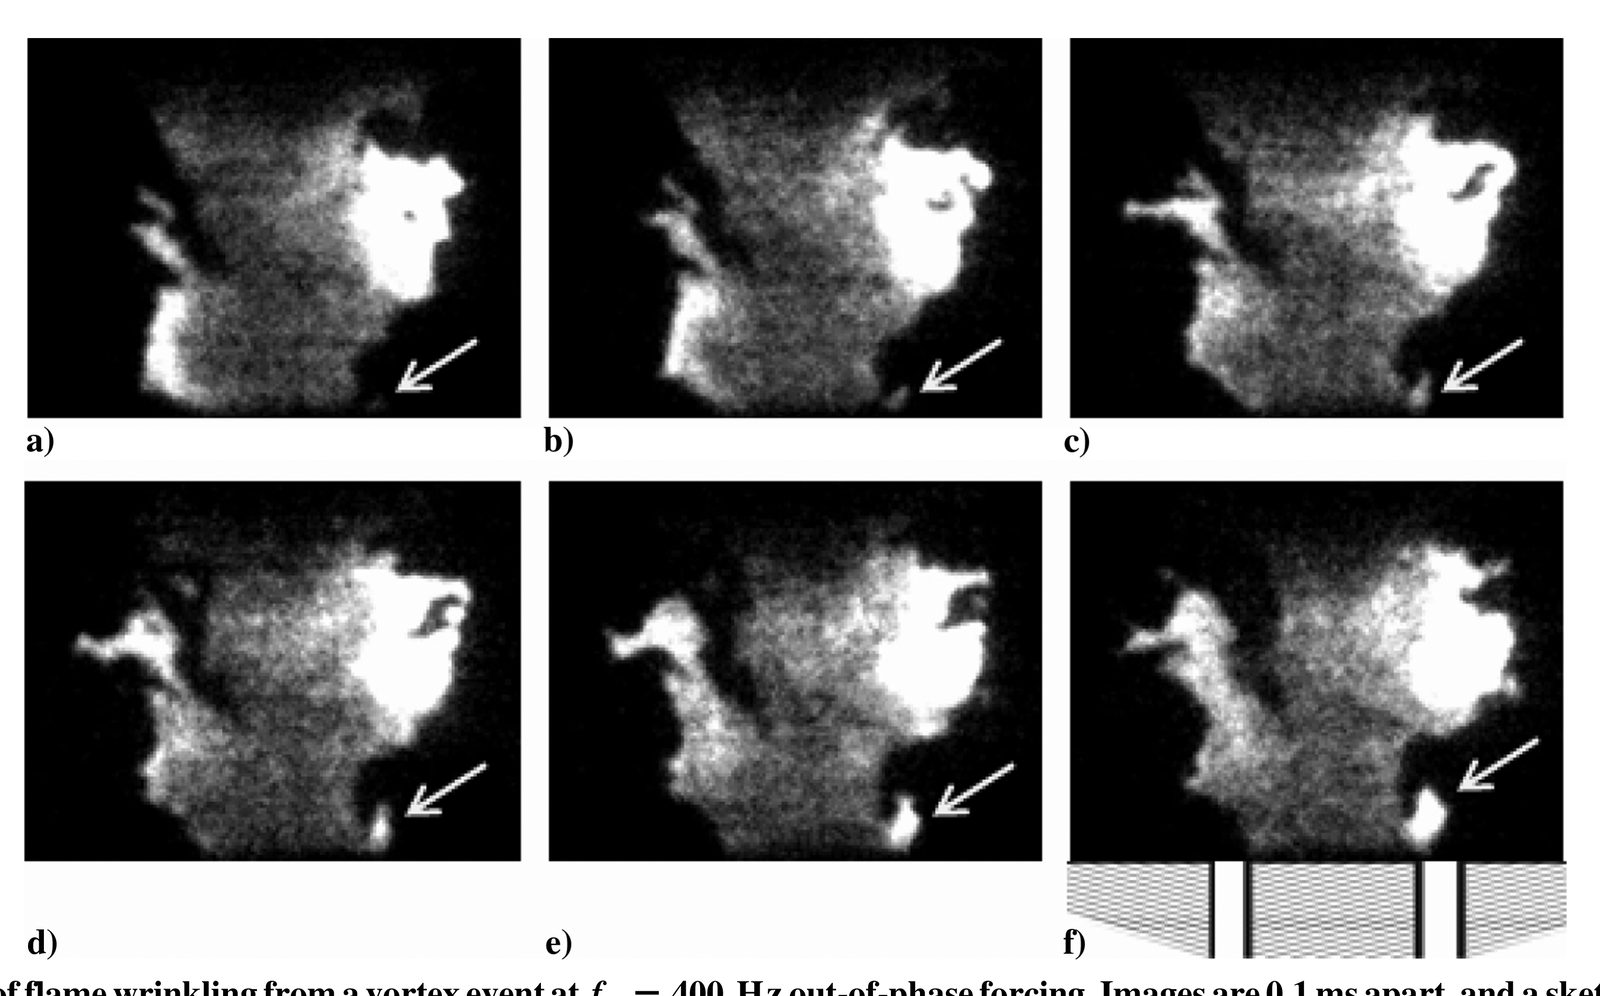
\includegraphics[width=1.000\linewidth]{figs/fig02.png}
\caption{横向声强迫下内剪切层涡形成事件与火焰响应（引自文献[8]）}
\end{figure}
综合来看，其一，现有研究对横流射流的涡系结构、轨迹弯曲与掺混特性已有较为清晰的认识；其二，对振荡横流与声学强迫条件下射流近场流动结构的响应也有一定积累；其三，针对横流火焰热释放率脉动的定量表征、以及其频域传递特性的研究仍相对有限，反应横向射流对谐波速度扰动的强迫响应也仅见零星报道[46]，可与旋流火焰结果相互对照的传递函数数据仍较缺乏。

\subsubsection{（二）TDLAS 燃烧诊断}
TDLAS 技术通过扫描分子吸收线型反演路径平均温度与组分柱浓度，其物理基础是 Beer-Lambert 定律与谱线强度、线型函数的温度依赖关系。Hanson 系统总结了定量激光传感器在化学动力学、推进与实用能源系统中的典型应用，明确了直接吸收光谱（direct absorption spectroscopy，DAS）与波长调制光谱（wavelength modulation spectroscopy，WMS）两类方法的适用边界[11]；Goldenstein 等对红外激光吸收光谱传感的理论基础、谱线参数数据库、线型拟合方法与工程实现进行了全面梳理，指出 Voigt 线型可同时描述多普勒展宽与碰撞展宽，是燃烧场谱线拟合的标准模型[12]；Allen 评述了二极管激光吸收传感器在气动与燃烧流场测量中的应用[13]。图 3 给出了 H\textsubscript{2}O 吸收线型的最佳拟合结果与线型参数随温度的变化规律[12]。

\begin{figure}[H]
\centering
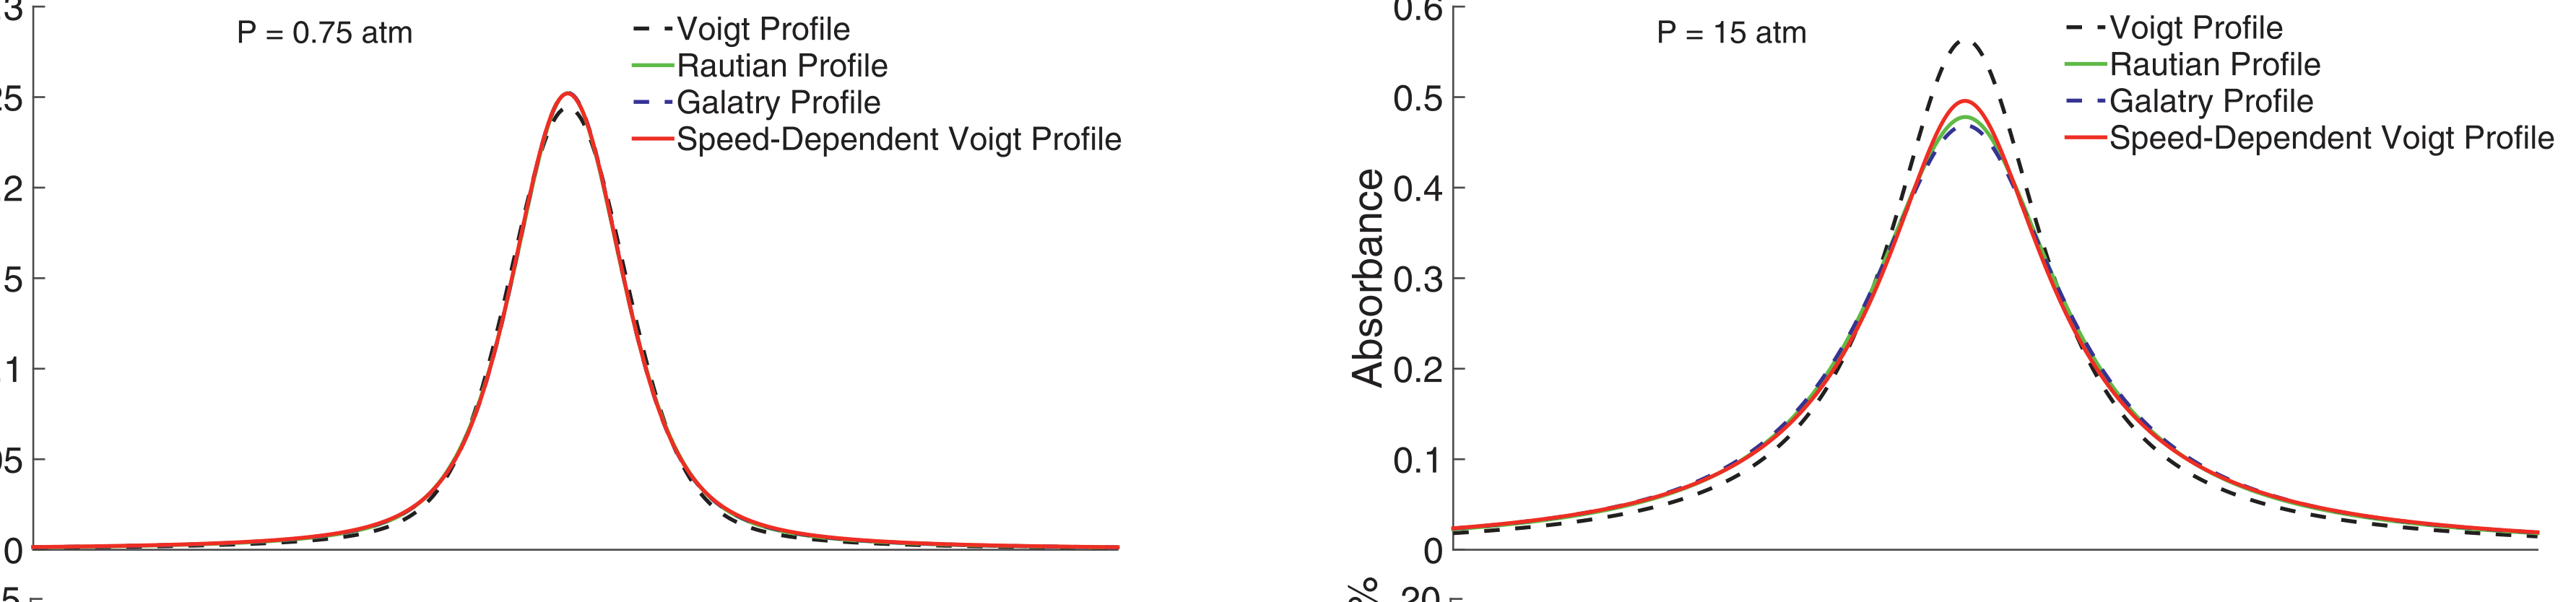
\includegraphics[width=1.000\linewidth]{figs/fig03.png}
\caption{H\textsubscript{2}O 吸收线型拟合与线型参数随温度的变化（引自文献[12]）}
\end{figure}
在测温方法上，多谱线方案与双线法是工程上最常用的两类手段。多谱线方案通过选取多条低态能级分布均匀的吸收线并采用玻尔兹曼图法反演温度，对谱线参数误差与环境干扰具有较好的容忍度；双线法则选取两条低态能级差较大的吸收线，通过两条谱线的积分吸收面积之比或峰值吸收之比反演温度，具有光路简单、响应快的优点，是动态燃烧场测量的首选方案[14]。在测量能力拓展方面，Sanders 等发展了可反演视线方向温度分布的二极管激光吸收传感器，通过多角度投影与反演算法获得了温度的空间分布[15]；Ma 等提出基于高光谱吸收光谱的层析成像方法，实现了温度与组分浓度的二维重建[16]。

近年来，层析反演与光路设计两方面均有明显进展。在反演算法方面，Liu 等提出基于非结构网格的激光吸收层析重建方法，通过自适应网格划分改善了有限投影视角下的重建精度与稳定性[17]；Zhao 等研制了兼顾稳定性与空间分辨率的激光吸收光谱层析传感器，并用于复杂燃烧火焰的诊断[18]；Yang 等基于紫外宽带吸收层析实现了轴对称火焰温度与 OH 浓度的二维定量重建[19]。在光路形式方面，为避免对穿式光路需要两侧开设光学窗口、多角度层析需要多组投影的局限，多光程池通过在有限空间内多次折返激光延长有效吸收光程，可显著提高弱吸收信号的探测灵敏度：Silver 系统比较了多种密集光斑多光程池结构，给出了光斑分布与光程长度的设计方法[20]；Kasyutich 与 Martin 采用两面柱面镜构建紧凑型多光程池并用于可调谐二极管激光吸收光谱测量，验证了圆柱面镜方案在小体积条件下的可行性[21]；Zhang 等提出了可变光程多光程池的设计方法，使有效光程可通过镜面间距按需调节[22]；Fendt 等将 Herriott 多光程池与单模光纤耦合超连续谱吸收光谱系统结合，在快速压缩膨胀机上实现了多种组分的同步定量诊断，验证了多光程光路在强振动、空间受限设备上的工程适用性[23]。上述光路形式与腔增强结构为受限空间下延长有效光程、提升信噪比提供了工程可行的技术路径[20,23]。图 4 给出了腔衰荡与离轴腔增强吸收光谱的光路布置示意[12]。

\begin{figure}[H]
\centering
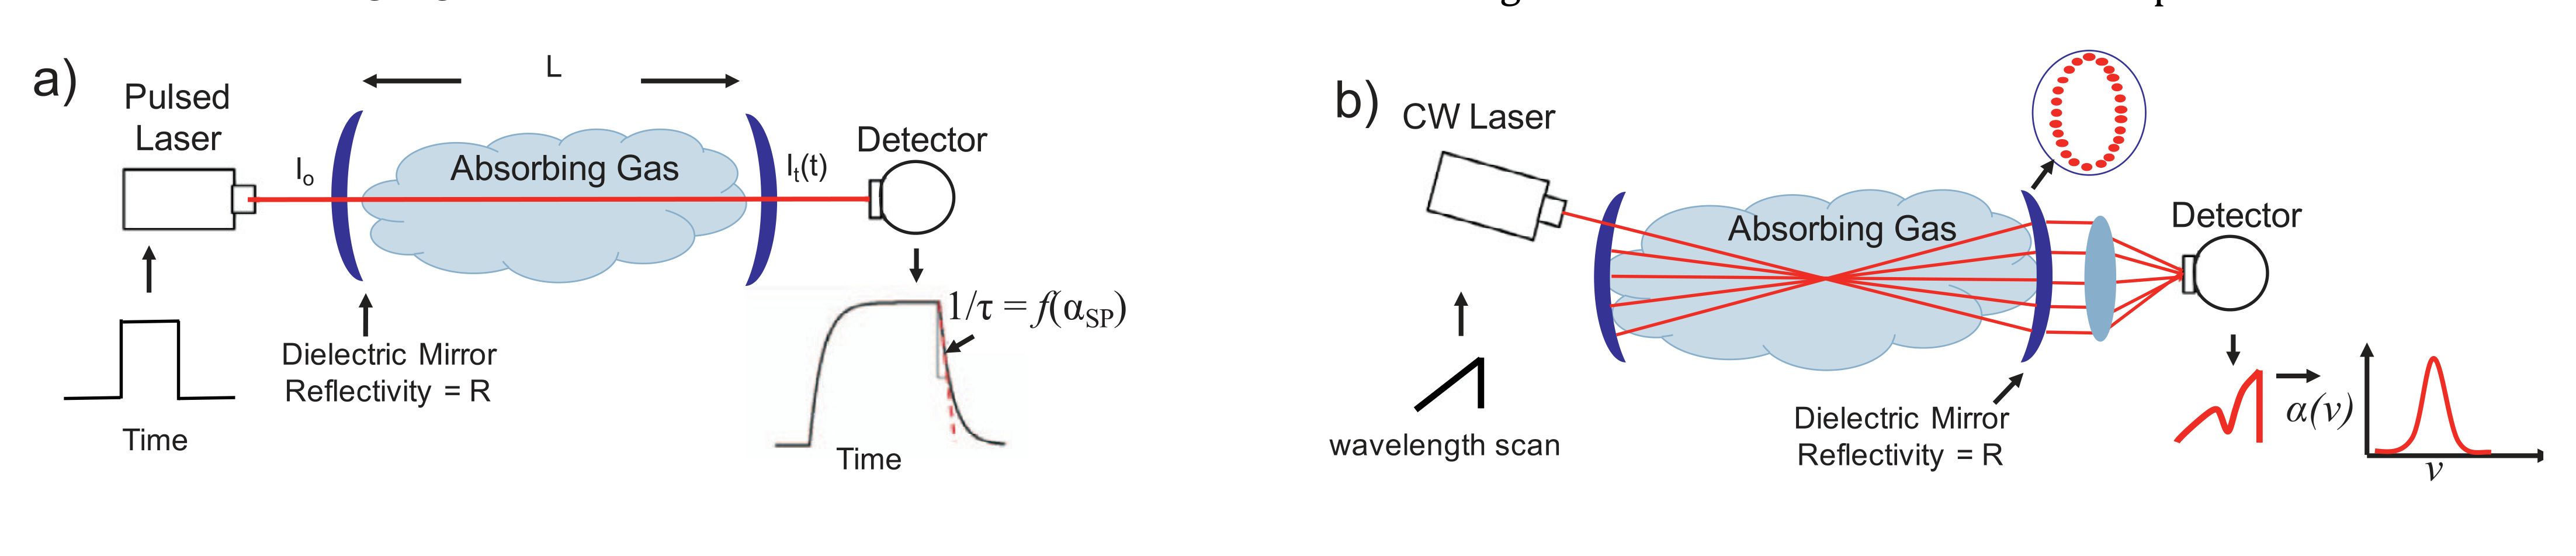
\includegraphics[width=1.000\linewidth]{figs/fig04.png}
\caption{腔衰荡与离轴腔增强吸收光谱光路示意（引自文献[12]）}
\end{figure}
在动态燃烧场测量方面，Liu 等采用中红外直接吸收光谱获得了声激励旋流火焰的时间分辨二维温度场，验证了 TDLAS 在非稳态燃烧场定量测量中的能力[14]。图 5 给出了不同声激励幅值下、不同相位时刻的火焰温度场演化结果[14]。

\begin{figure}[H]
\centering
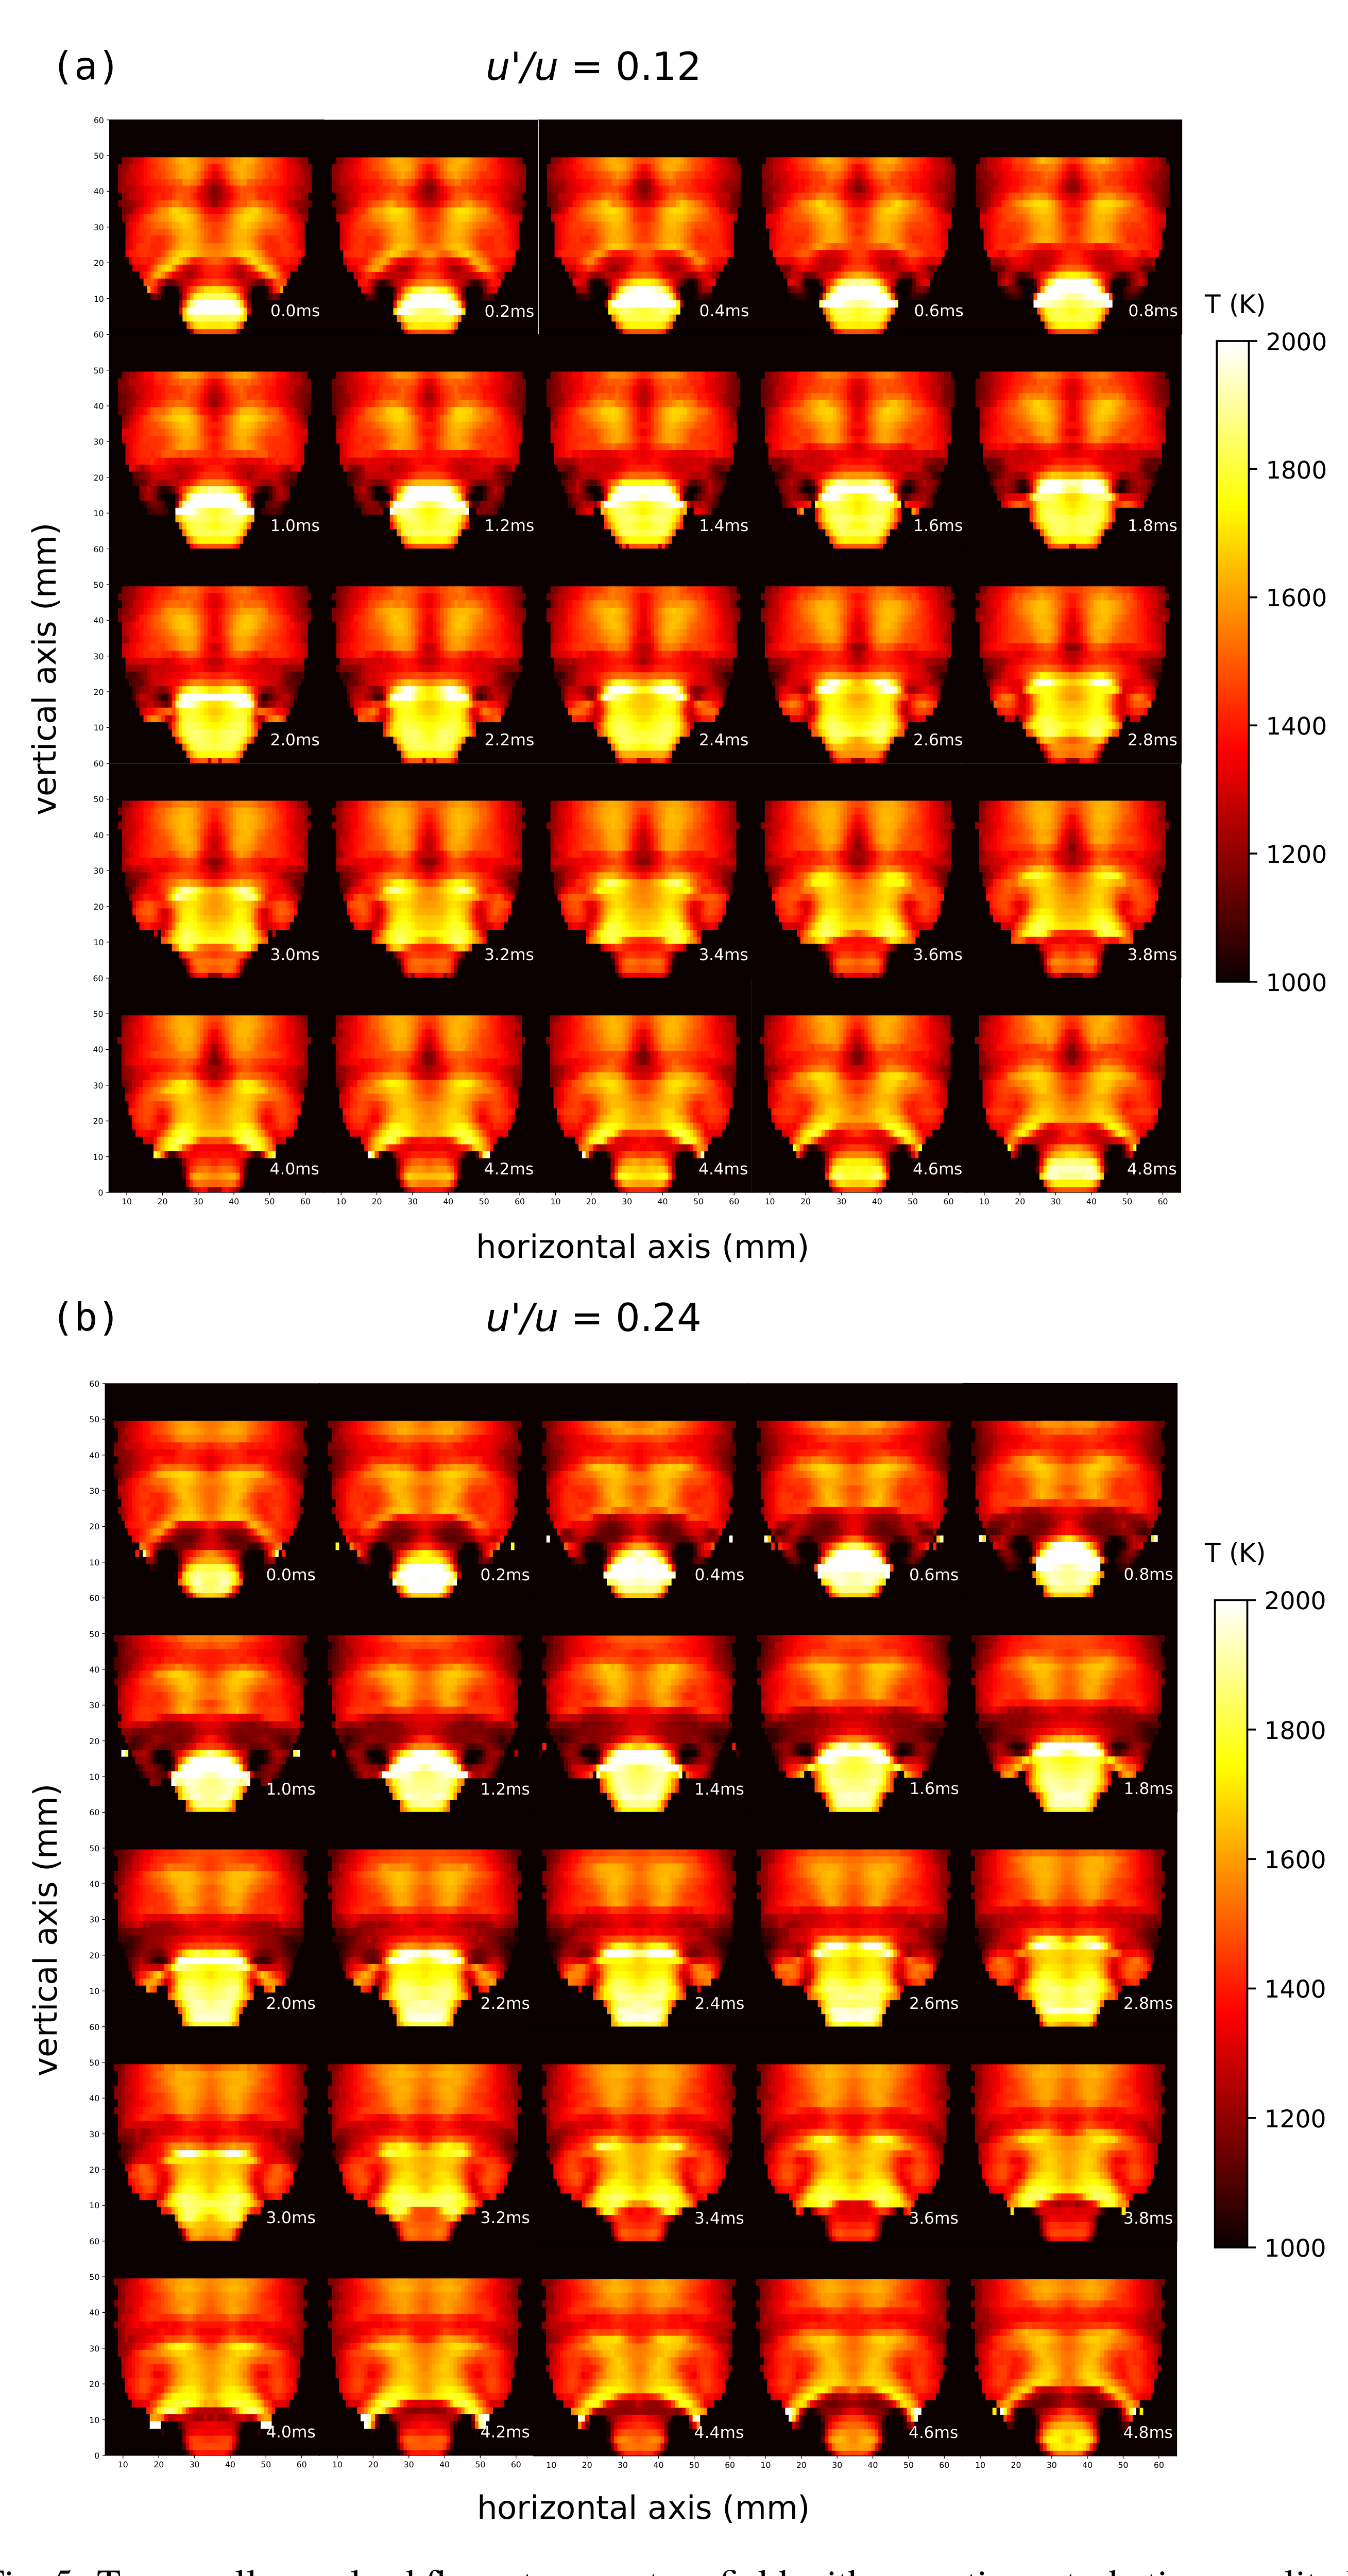
\includegraphics[width=0.673\linewidth]{figs/fig05.png}
\caption{声激励旋流火焰的时间分辨二维温度场（引自文献[14]）}
\end{figure}
综合来看，其一，TDLAS 的理论基础与谱线拟合方法已较为成熟，双线法测温在工程上应用广泛；其二，层析反演与多光程光路的发展使 TDLAS 正由单点/单线走向二维、高灵敏度测量；其三，现有反射式/多光程光路研究多面向痕量气体检测或长光程吸收池，将多光程光路与自发光高速摄影结合、用于横流火焰“同步、同光路”定量诊断的系统性工作报道较少。

\subsubsection{（三）火焰自发光成像与融合测量}
火焰自发光成像通过捕获 CH*（约 430 nm）、OH*（约 310 nm）等自由基的化学发光信号获得火焰二维结构，具有设备简单、时空分辨高的突出优势，是燃烧不稳定性研究中应用最广泛的诊断手段之一。然而，自发光强度是温度、组分浓度与光学收集效率的复杂函数，单独使用时难以实现定量测量，通常只能反映热释放率脉动的相对变化[26,28]。

在自发光信号定量化方面，Hardalupas 等系统评估了化学发光传感器用于测量局部热释放率与当量比时的空间分辨率，量化了成像系统点扩散函数对定量精度的影响，并给出了传感器设计准则[24]；Hardalupas 与 Orain 进一步利用火焰化学发光发射实现了热释放率与当量比脉动的局部测量，讨论了 CH*/OH* 信号比与热释放率之间的对应关系[27]；Lee 与 Santavicca 系统评述了贫预混燃烧室中基于化学发光的诊断方法及其在燃烧不稳定性研究中的应用，认为化学发光方法的关键限制在于其标定依赖[26]；Moroshkina 等在平面多孔燃烧器上研究了甲烷-空气火焰的化学发光光谱特性，建立了自发光强度与火焰温度、当量比之间的经验关联[25]。图 6 给出了化学发光强度随预混度与当量比的变化规律[26]。

\begin{figure}[H]
\centering
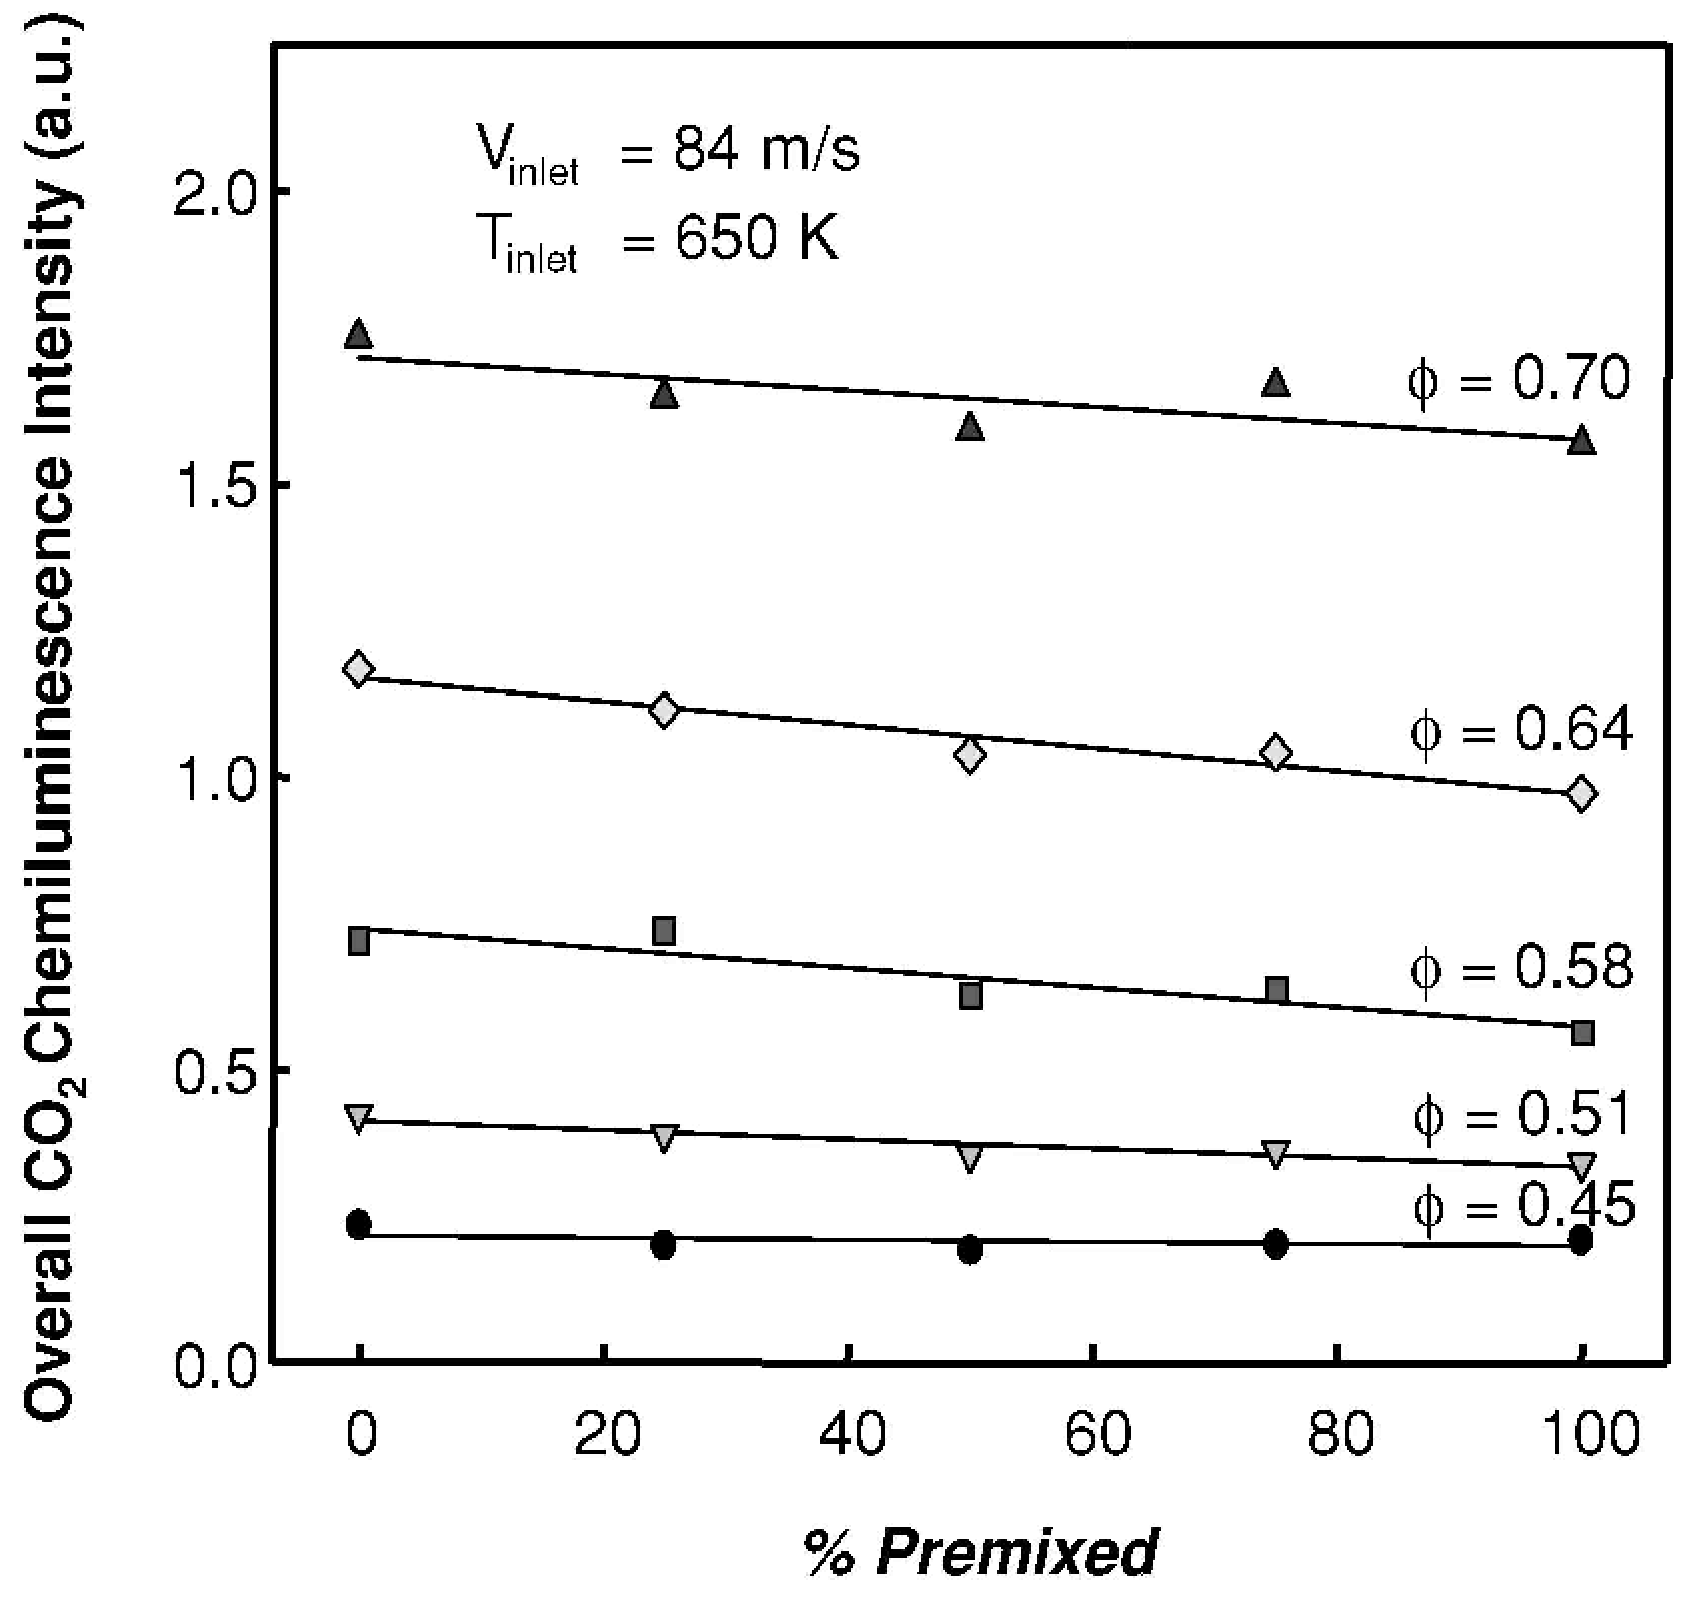
\includegraphics[width=1.000\linewidth]{figs/fig06.png}
\caption{化学发光强度随预混度与当量比的变化（引自文献[26]）}
\end{figure}
在融合测量思路方面，以激光诊断提供定量基准、以自发光成像提供空间结构，二者互补，已成为燃烧诊断的重要发展方向。本课题组已在反射式 TDLAS 与 PIV/PLIF 同时拍摄装置方面提交发明专利申请，为“同光路、同步”融合测量提供了硬件基础[29]。

\subsubsection{（四）火焰传递函数测量}
火焰传递函数描述热释放率脉动对来流速度脉动的增益与相位响应，通常定义为 FTF(ω)=q′(ω)/q̄ 与 u′(ω)/ū 之比，是低阶热声网络模型的关键输入，也是预测与抑制燃烧不稳定性的核心物理模型[30]。Candel 围绕燃烧动力学与控制、旋流火焰动力学等方向开展了大量开创性工作，建立了从火焰响应函数到燃烧室声学耦合的完整分析链条[32-34]；Palies 等给出了预混受限旋流火焰动力学特性的系统结果，并进一步发展了旋流器与湍流预混旋流火焰的联合动力学模型[35-36]。

在理论框架方面，Ducruix 等归纳了燃烧不稳定性的基本耦合与驱动机制，明确了速度脉动—热释放率脉动—声压脉动的闭环耦合路径[30]；Schuller 等建立了层流火焰传递函数的统一预测模型，给出了锥形火焰与 V 形火焰的增益与相位随频率变化的解析表达，指出增益在中低频趋近于 1、相位随时间延迟近似线性滞后，是本课题 FTF 提取的目标形式[31]。图 7 给出了不同火焰角下层流锥形火焰的传递函数增益与相位曲线[31]。

\begin{figure}[H]
\centering
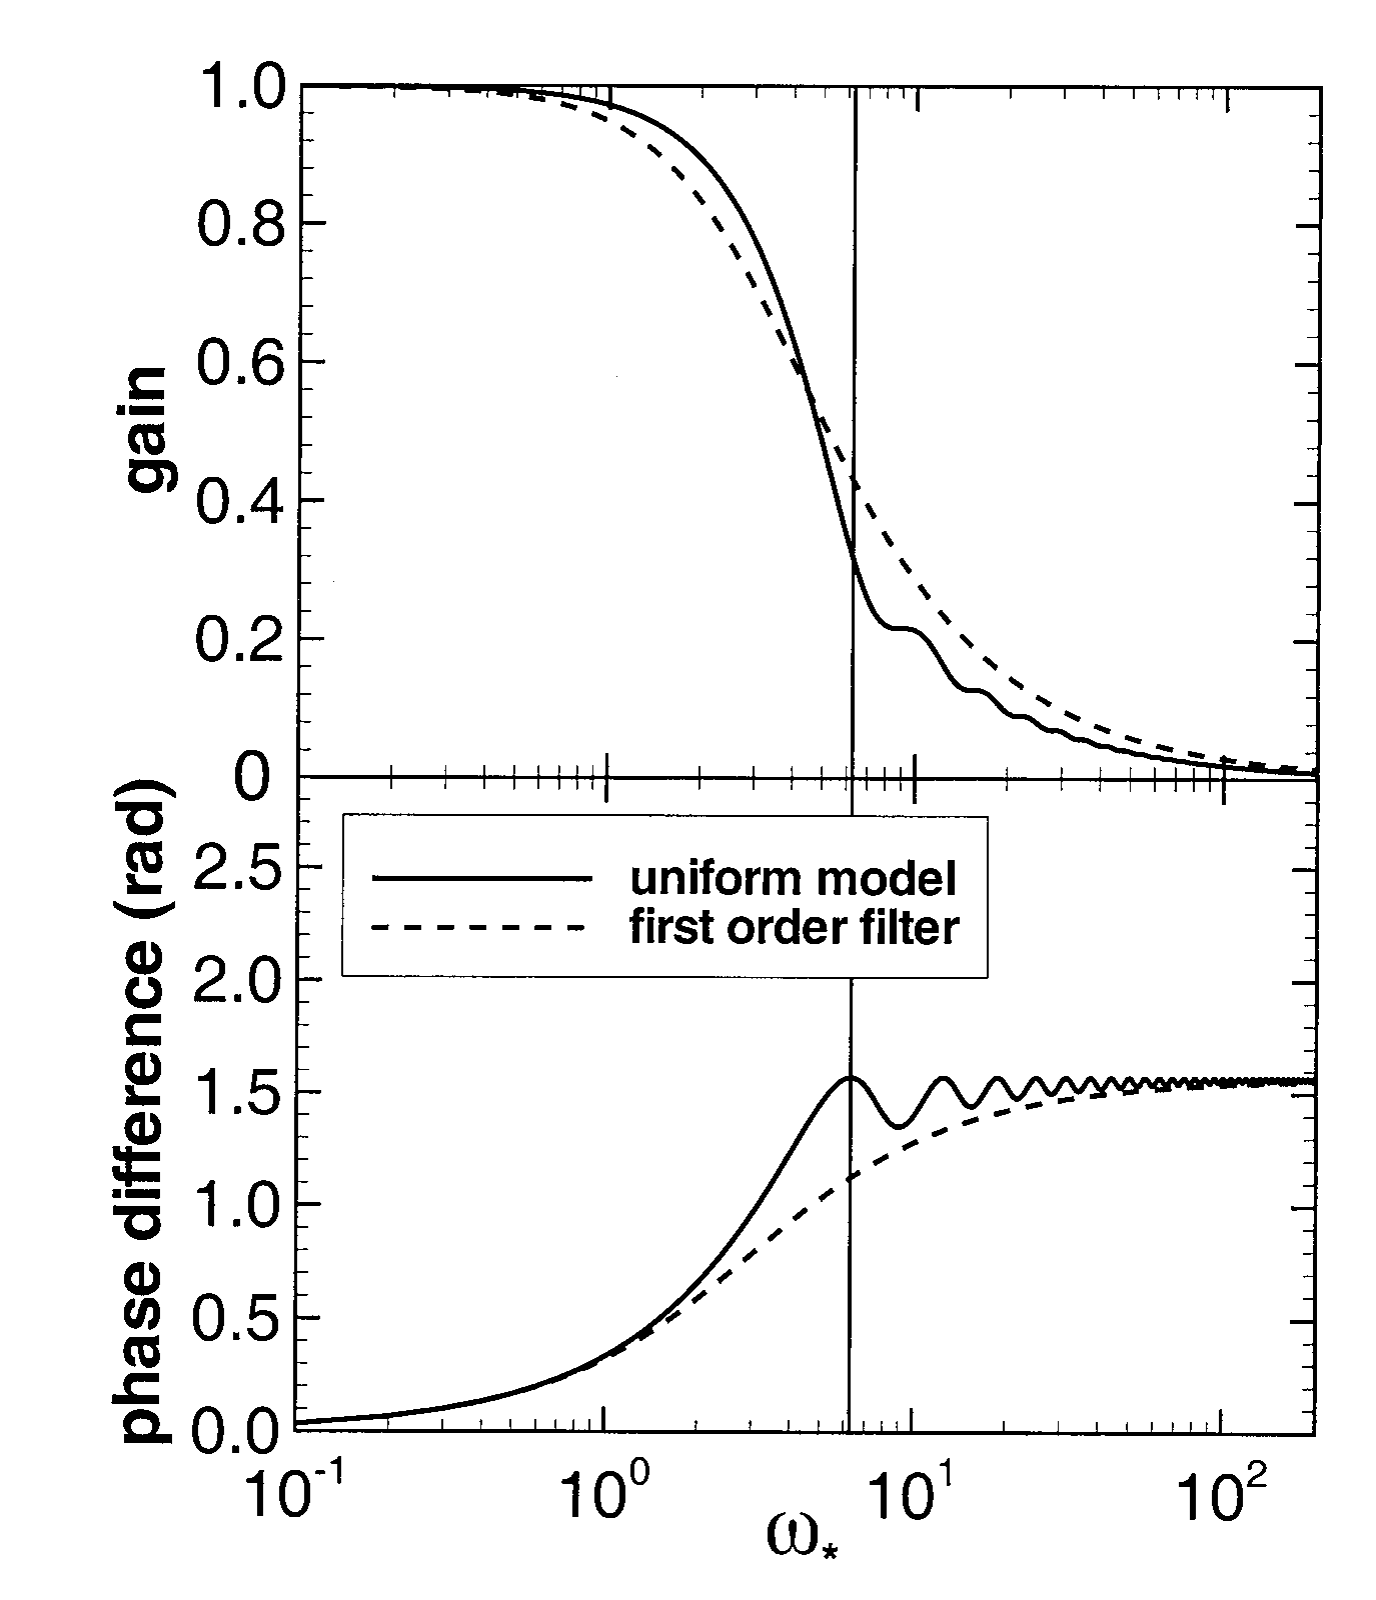
\includegraphics[width=0.819\linewidth]{figs/fig07.png}
\caption{层流火焰传递函数的增益与相位特性（引自文献[31]）}
\end{figure}
在非线性刻画方面，Bailly 等对火焰传递函数与描述函数理论作了专门评述，指出线性 FTF 仅在小扰动条件下成立[37]；Wang 等将二维波基低阶网络模型用于环形燃烧室极限环预测与声耗散率量化，实现了从 FDF 到极限环幅值的预测[38]；Ji 等系统研究了燃气轮机燃烧室中不同钝体阻塞比下旋流火焰在声强迫作用下的非线性响应，表明激励幅值增大后火焰增益出现饱和、相位发生畸变，火焰卷曲、褶皱乃至夹断等非线性行为凸显，需采用火焰描述函数刻画，并耦合燃烧室声学模型预测极限环[42]。图 8 给出了不同激励幅值下火焰形态与响应的演化过程[42]。

\begin{figure}[H]
\centering
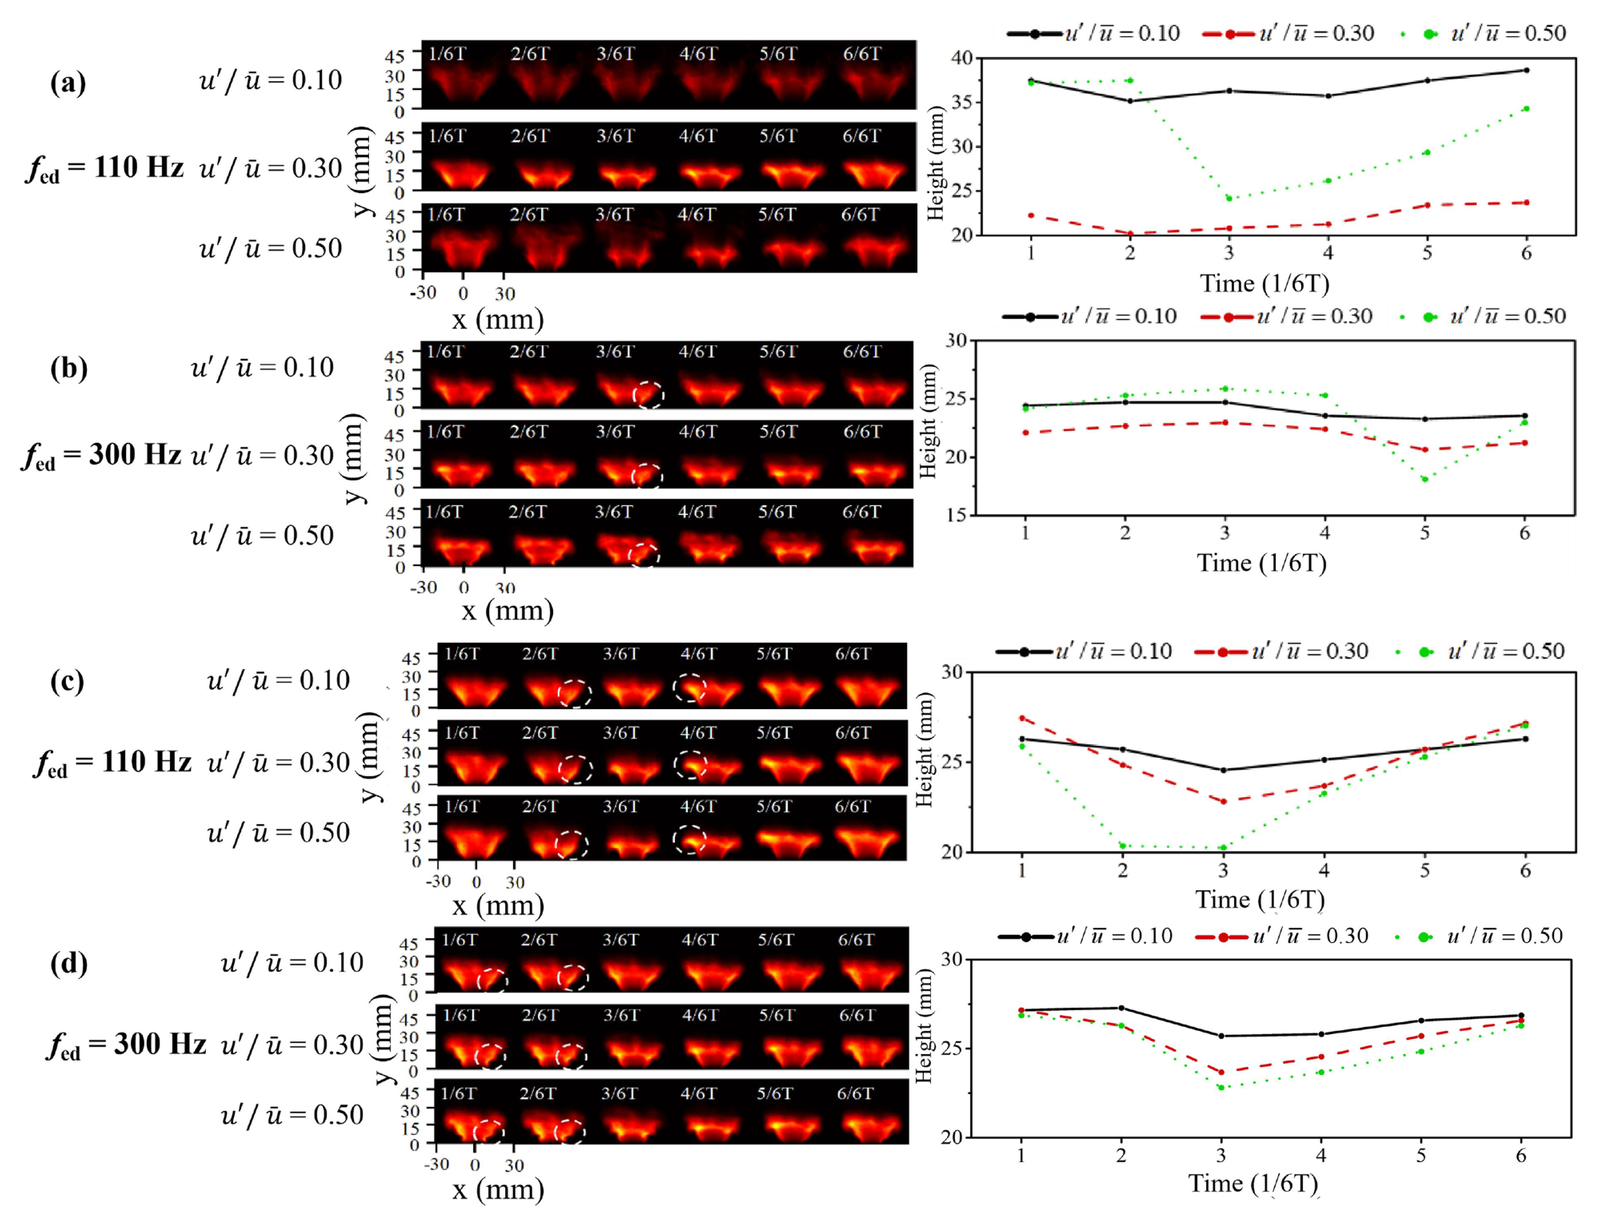
\includegraphics[width=1.000\linewidth]{figs/fig08.png}
\caption{不同激励幅值下的火焰形态演化与响应（引自文献[42]）}
\end{figure}
在定量测量手段方面，Dharmaputra 等采用多麦克风、OH* 成像、TDLAS 与延迟时间分布模型等多手段同步测量级联燃烧室的 FTF，展示了多方法交叉验证的价值，并给出了燃烧室级 FTF 随燃料氢含量变化的系统结果[43]。图 9 给出了级联燃烧室中 OH* 平均化学发光图像与相应 FTF 增益、相位随下游位置的变化[43]。

\begin{figure}[H]
\centering
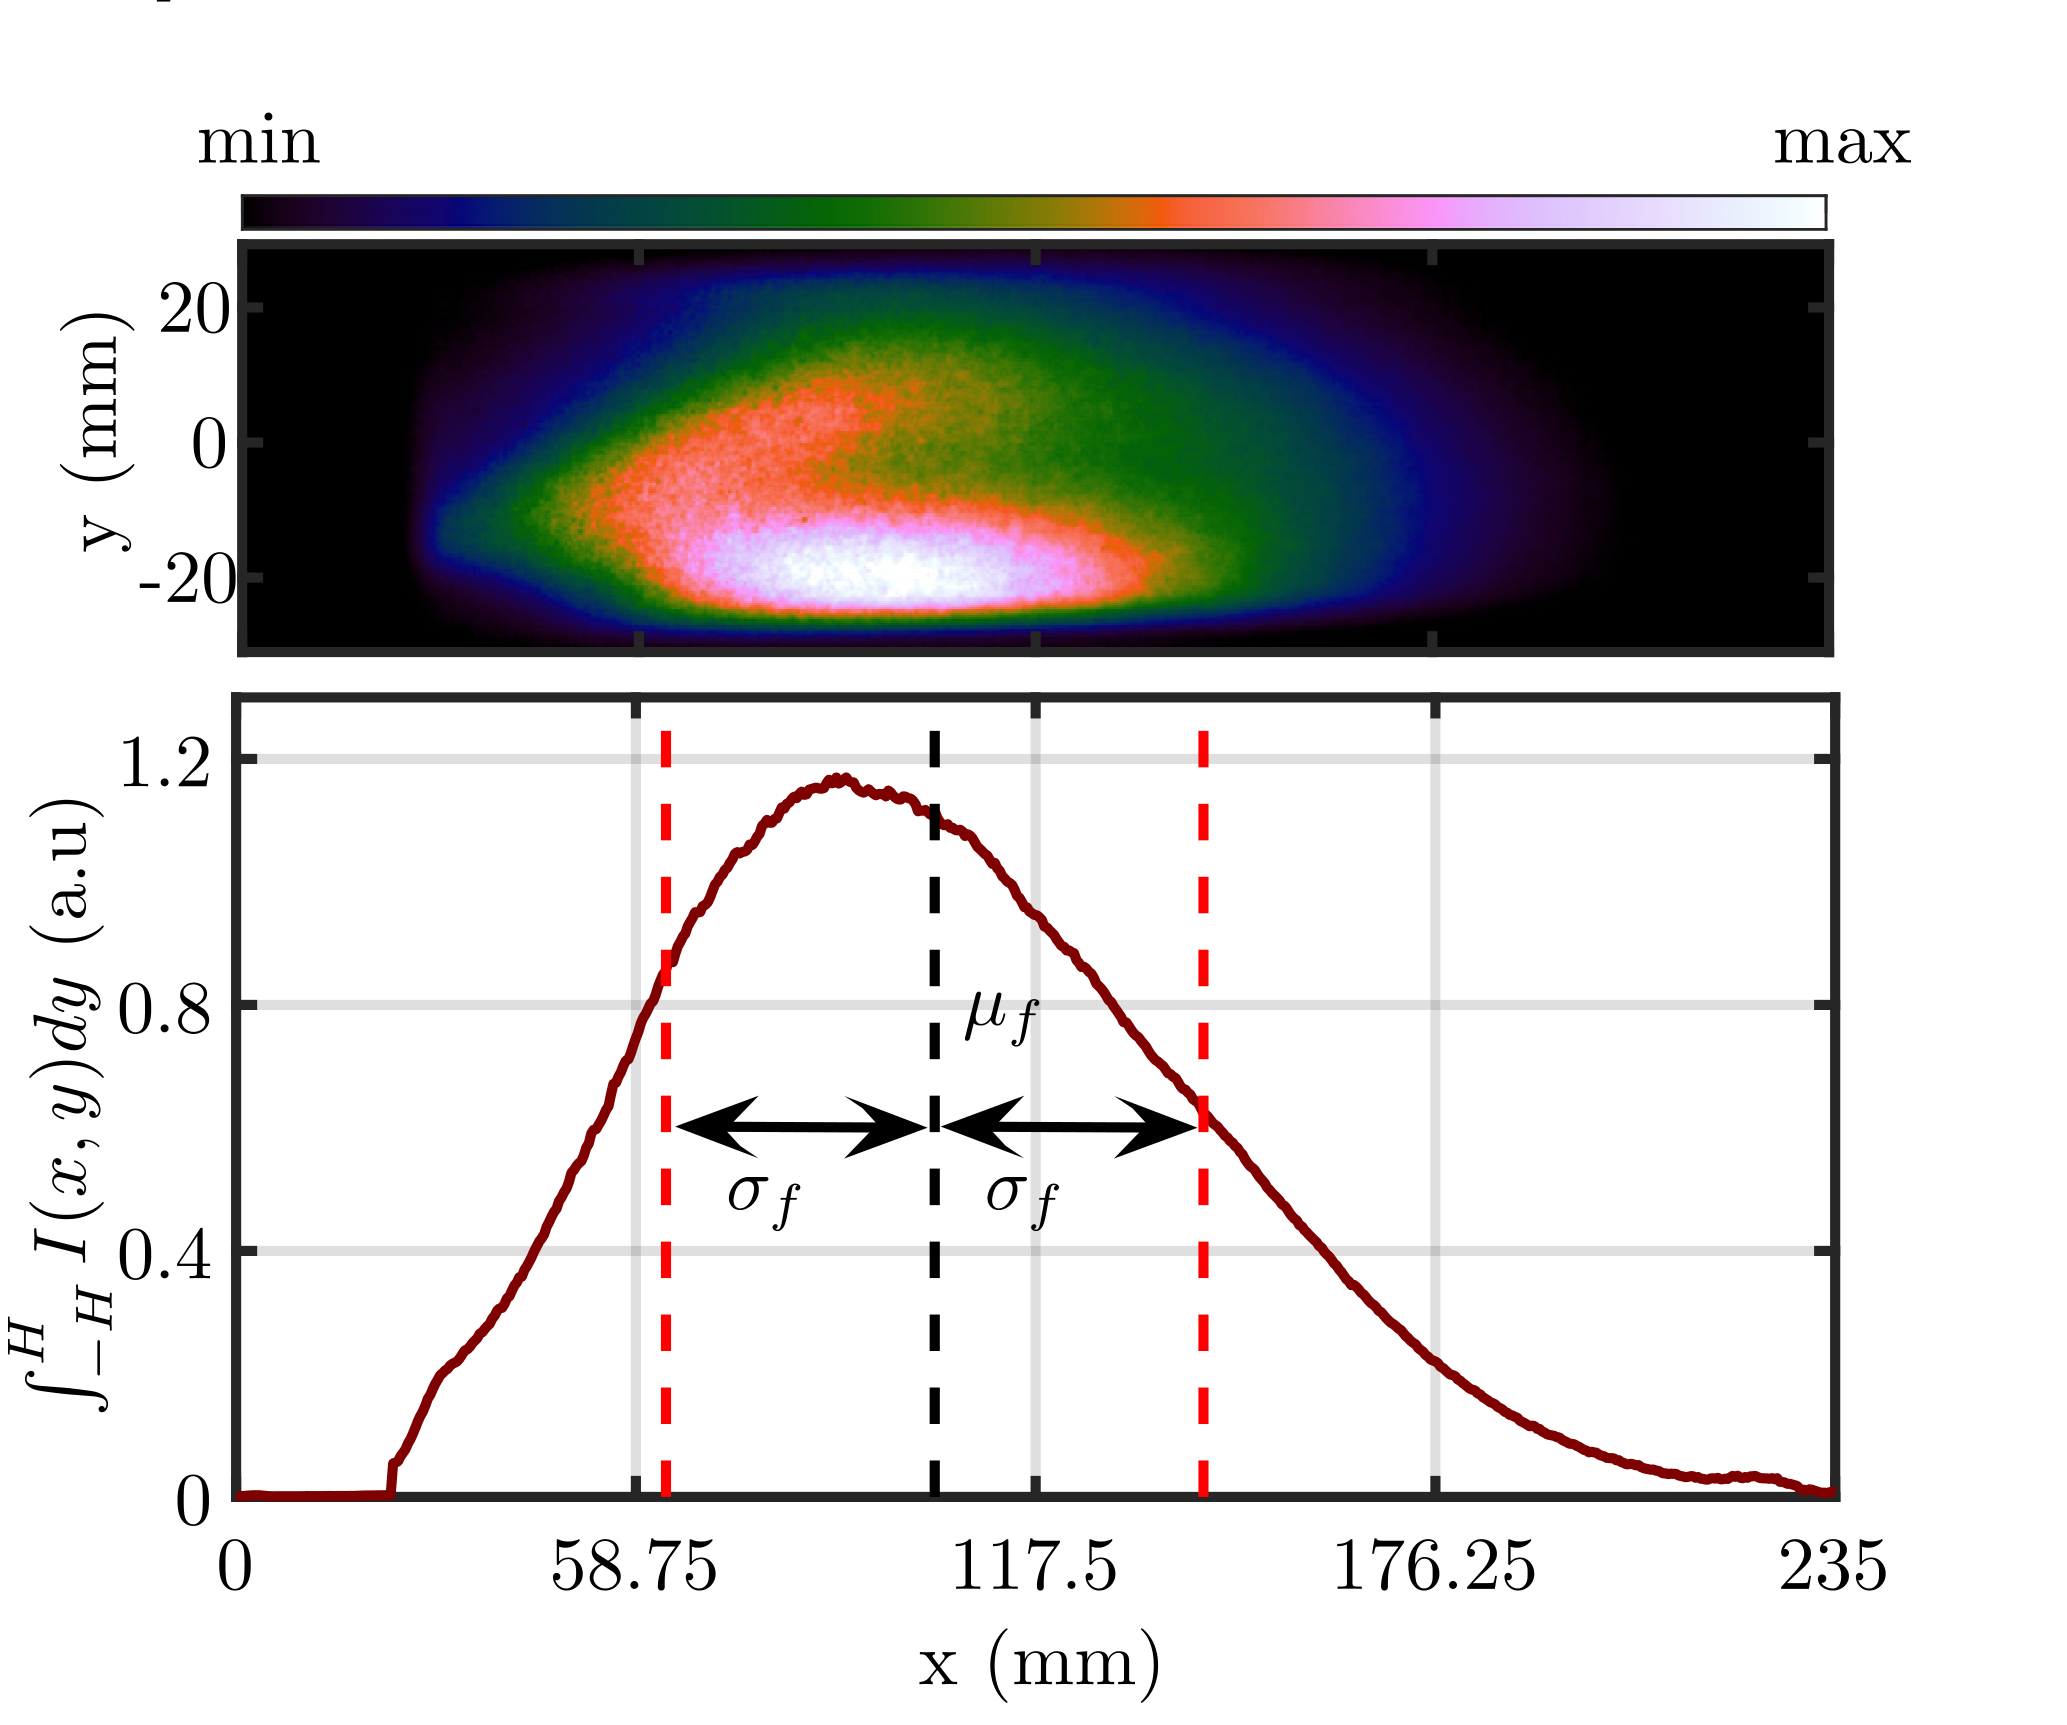
\includegraphics[width=1.000\linewidth]{figs/fig09.png}
\caption{级联燃烧室 OH* 化学发光与火焰传递函数（引自文献[43]）}
\end{figure}
国内方面，张金锋等对氢混燃料旋流预混火焰的传递函数开展了实验研究，获得了增益与相位随氢含量的变化规律[44]；王子豫与朱彤对燃气燃烧热声不稳定的机理、表征方法与抑制手段进行了系统梳理，指出工况参数与燃料组分是影响火焰响应的关键因素[45]。此外，Poinsot[39]、Lieuwen[40]与 Dowling 等[41]分别从工程预测、非定常燃烧室物理与燃烧噪声角度给出了系统性框架，为本课题的实验设计与数据处理提供了理论参照。

在速度脉动测量方面，热线风速仪、激光多普勒测速与双麦克风声学反演是三类主流手段。热线风速仪直接测量速度脉动，频响高、成本低，但需解决高温环境下的探头污染与标定问题[58-60]；Vishnyakov 等在激波/边界层干扰区对比了热线风速仪与粒子图像测速结果，指出热线风速仪的频响优势在强非定常流动测量中不可替代，但其标定关系对温度与污染高度敏感[47]；激光多普勒测速为绝对测量、无需标定，但系统复杂、成本高。综合来看，其一，现有 FTF 研究几乎全部集中于旋流火焰，横向射流火焰的 FTF 系统测量数据缺乏[46]；其二，速度脉动测量多依赖多麦克风声学反演，存在间接性与假设依赖性，采用热线风速仪直接测量的方案尚不多见；其三，多手段交叉验证（多麦克风+OH* 成像+TDLAS+热线）的实验范式值得在本课题中借鉴[43-44]。

\subsubsection{（五）熄火主动控制}
贫油熄火是限制燃烧室低排放运行的主要障碍，主动控制是拓宽稳定运行边界的有效途径。McManus 等最早系统评述了燃烧不稳定性的主动控制方法，奠定了开环与闭环控制的分类框架，并指出闭环控制的关键在于可靠的前兆传感器[48]；Docquier 等对燃烧控制与传感技术进行了系统综述，比较了压力、化学发光与光学传感器在控制回路中的适用性[49]。

在熄火前兆判别方面，Nair 与 Lieuwen 研究了预混火焰熄火过程中的声学特征，指出压力脉动低频段的功率份额在熄火前显著上升，可作为熄火前兆[50]；Yi 与 Gutmark 提出了基于压力与化学发光信号统计特征的贫油熄火实时预测方法，在燃气轮机燃烧器上实现了提前预警[51]；Zhang 等进一步利用火焰图像形态特征实现了旋流火焰贫油熄火的预测，表明图像特征与熄火裕度之间存在稳定映射[52]；Muruganandam 等提出了基于化学发光与声学信号特征融合的贫油熄火主动控制方法[53]；Morales 等提出了预测稳定预混火焰贫油熄火边界的统一 Karlovitz 数判据，为熄火极限的理论预估提供了依据[10]。

在激光传感闭环控制方面，最具代表性的是 Li 等利用可调谐二极管激光温度传感器，提出 FFT\%[0-50] 熄火前兆指标，在旋流稳定燃烧器上实现了主动贫油熄火闭环控制：控制值在熄火前显著上升，控制开启后回落，证明了 TDLAS 传感器用于燃烧主动控制的可行性[54]。图 10 给出了该闭环控制实验的传感器与锁相 2f 检测链路[54]，图 11 给出了 FFT\%[0-50] 熄火前兆指标随当量比的变化[54]。

\begin{figure}[H]
\centering
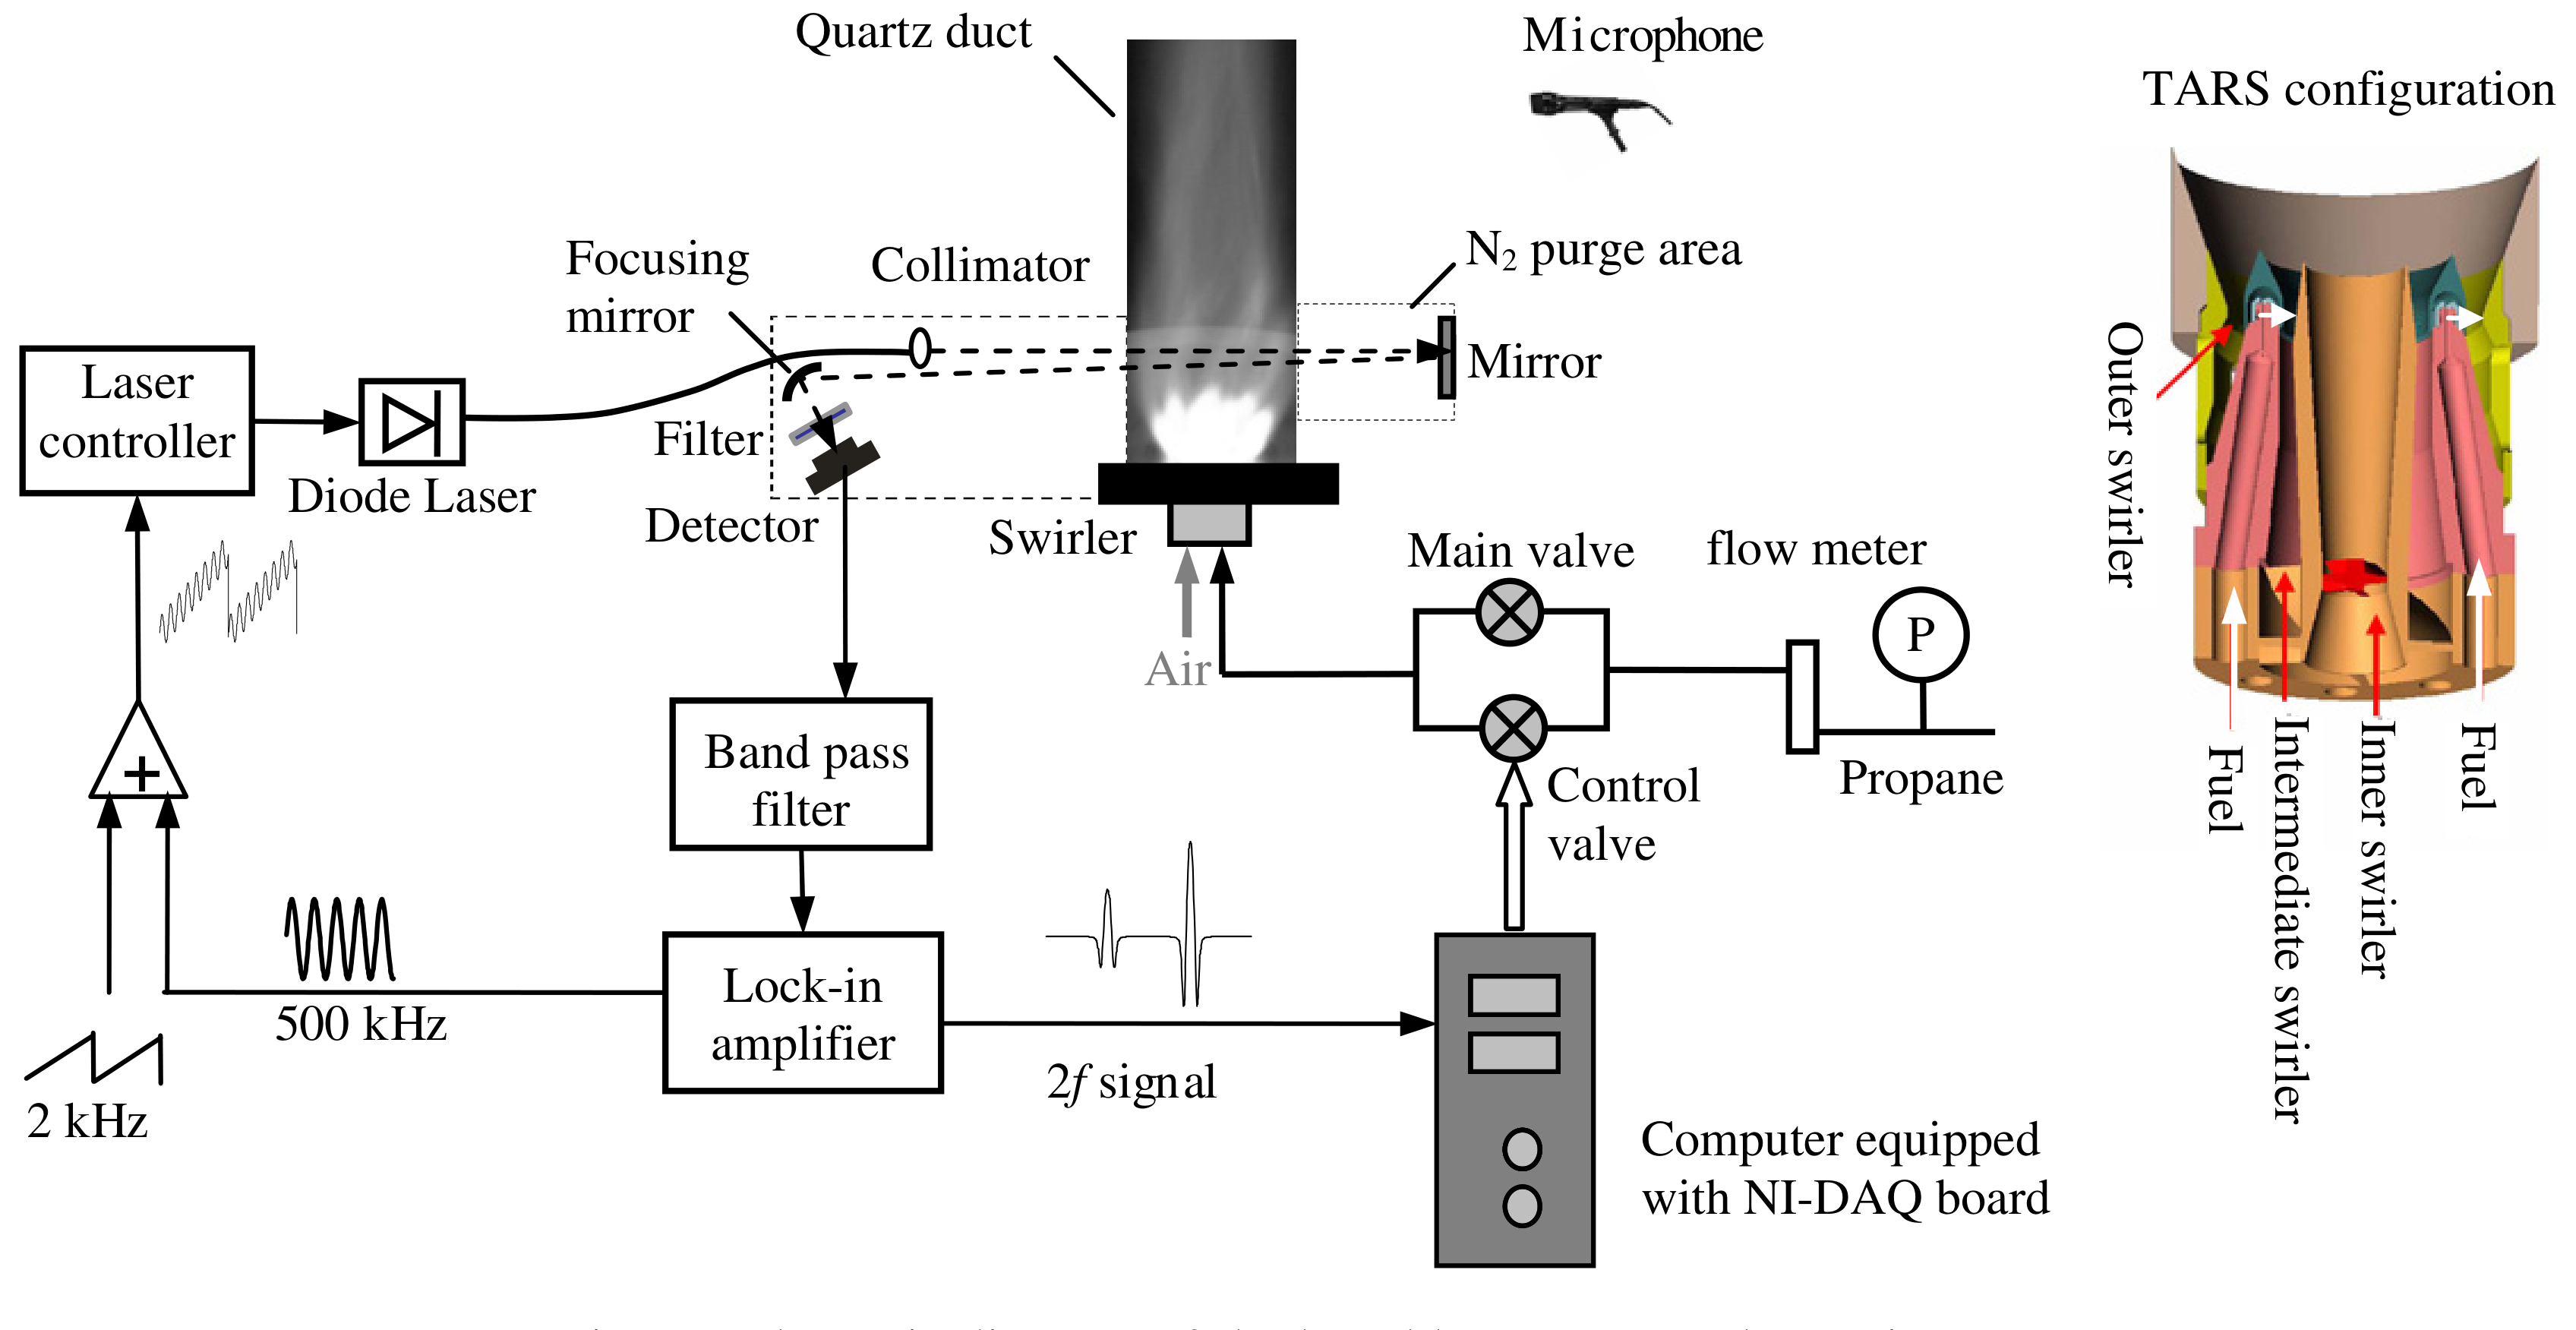
\includegraphics[width=1.000\linewidth]{figs/fig10.png}
\caption{TDLAS 传感器与锁相 2f 检测链路（引自文献[54]）}
\end{figure}
\begin{figure}[H]
\centering
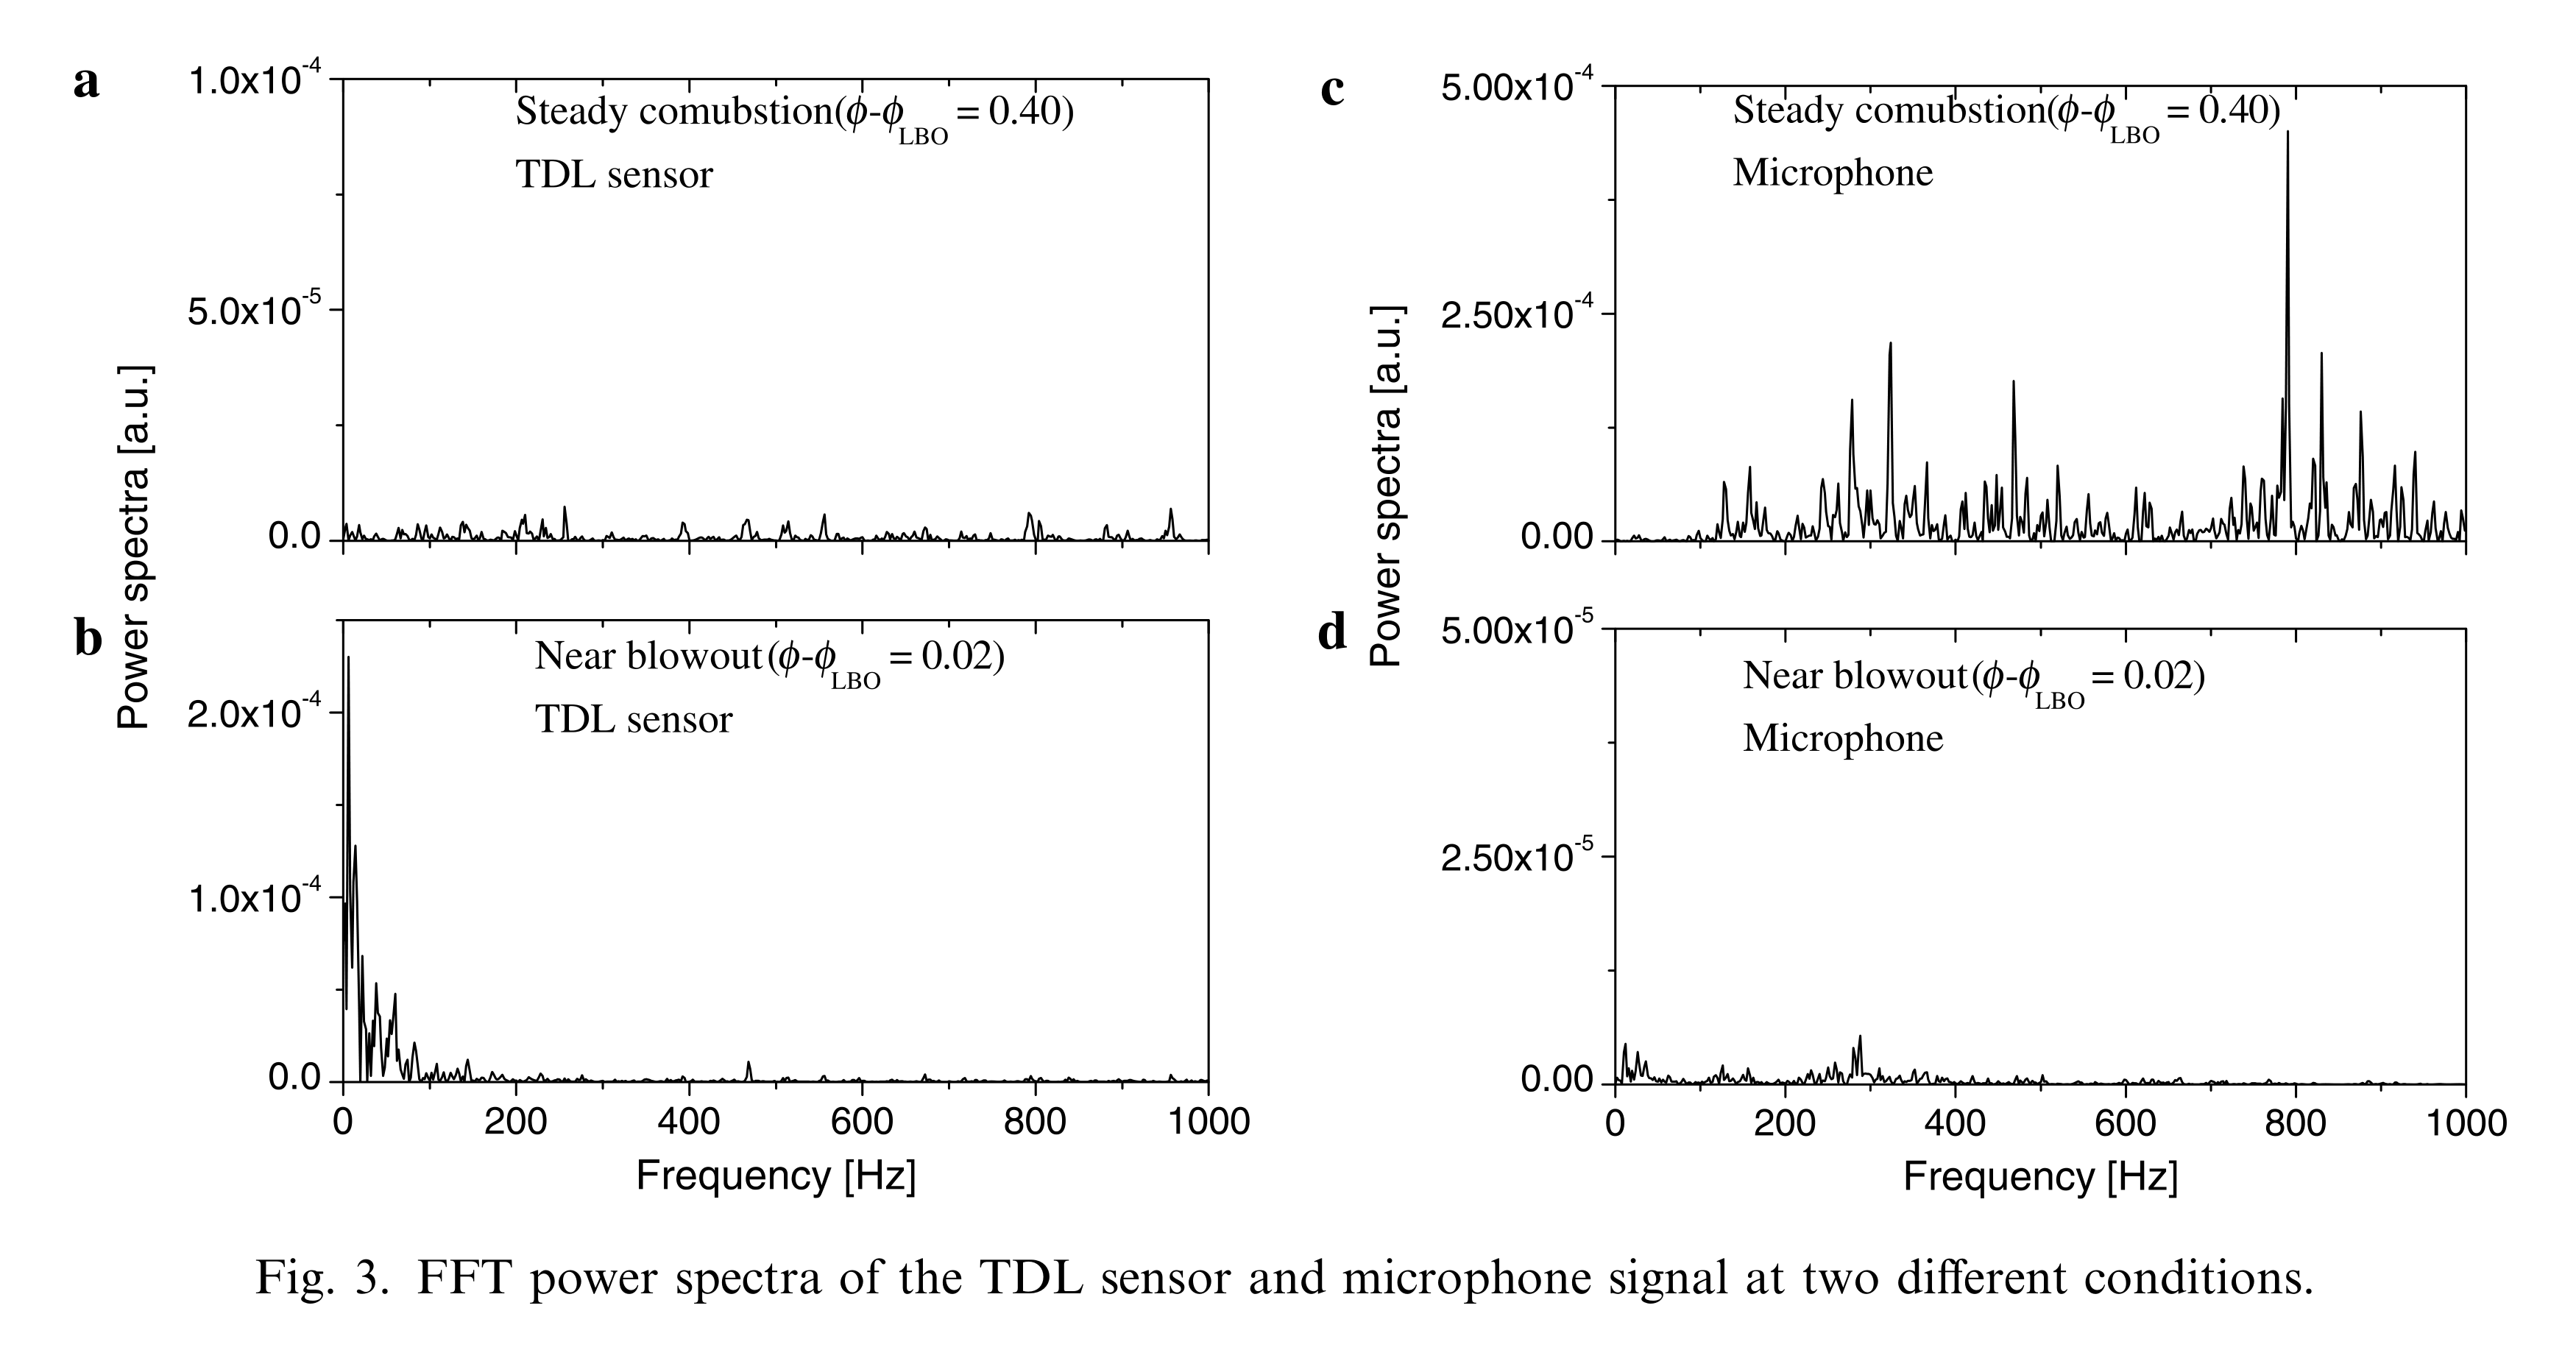
\includegraphics[width=1.000\linewidth]{figs/fig11.png}
\caption{FFT\%[0-50] 熄火前兆指标随当量比的变化（引自文献[54]）}
\end{figure}
在控制逻辑实现方面，Muruganandam 等提出的控制算法采用事件计数与定时器配合的方式：若无熄火事件发生则逐步降低引燃燃料比例，一旦检测到离散熄火事件即按事件次数成比例地增加引燃比例，从而在保证安全裕度的前提下尽可能维持低排放运行[53]。图 12 给出了该控制逻辑的判断流程[53]。

\begin{figure}[H]
\centering
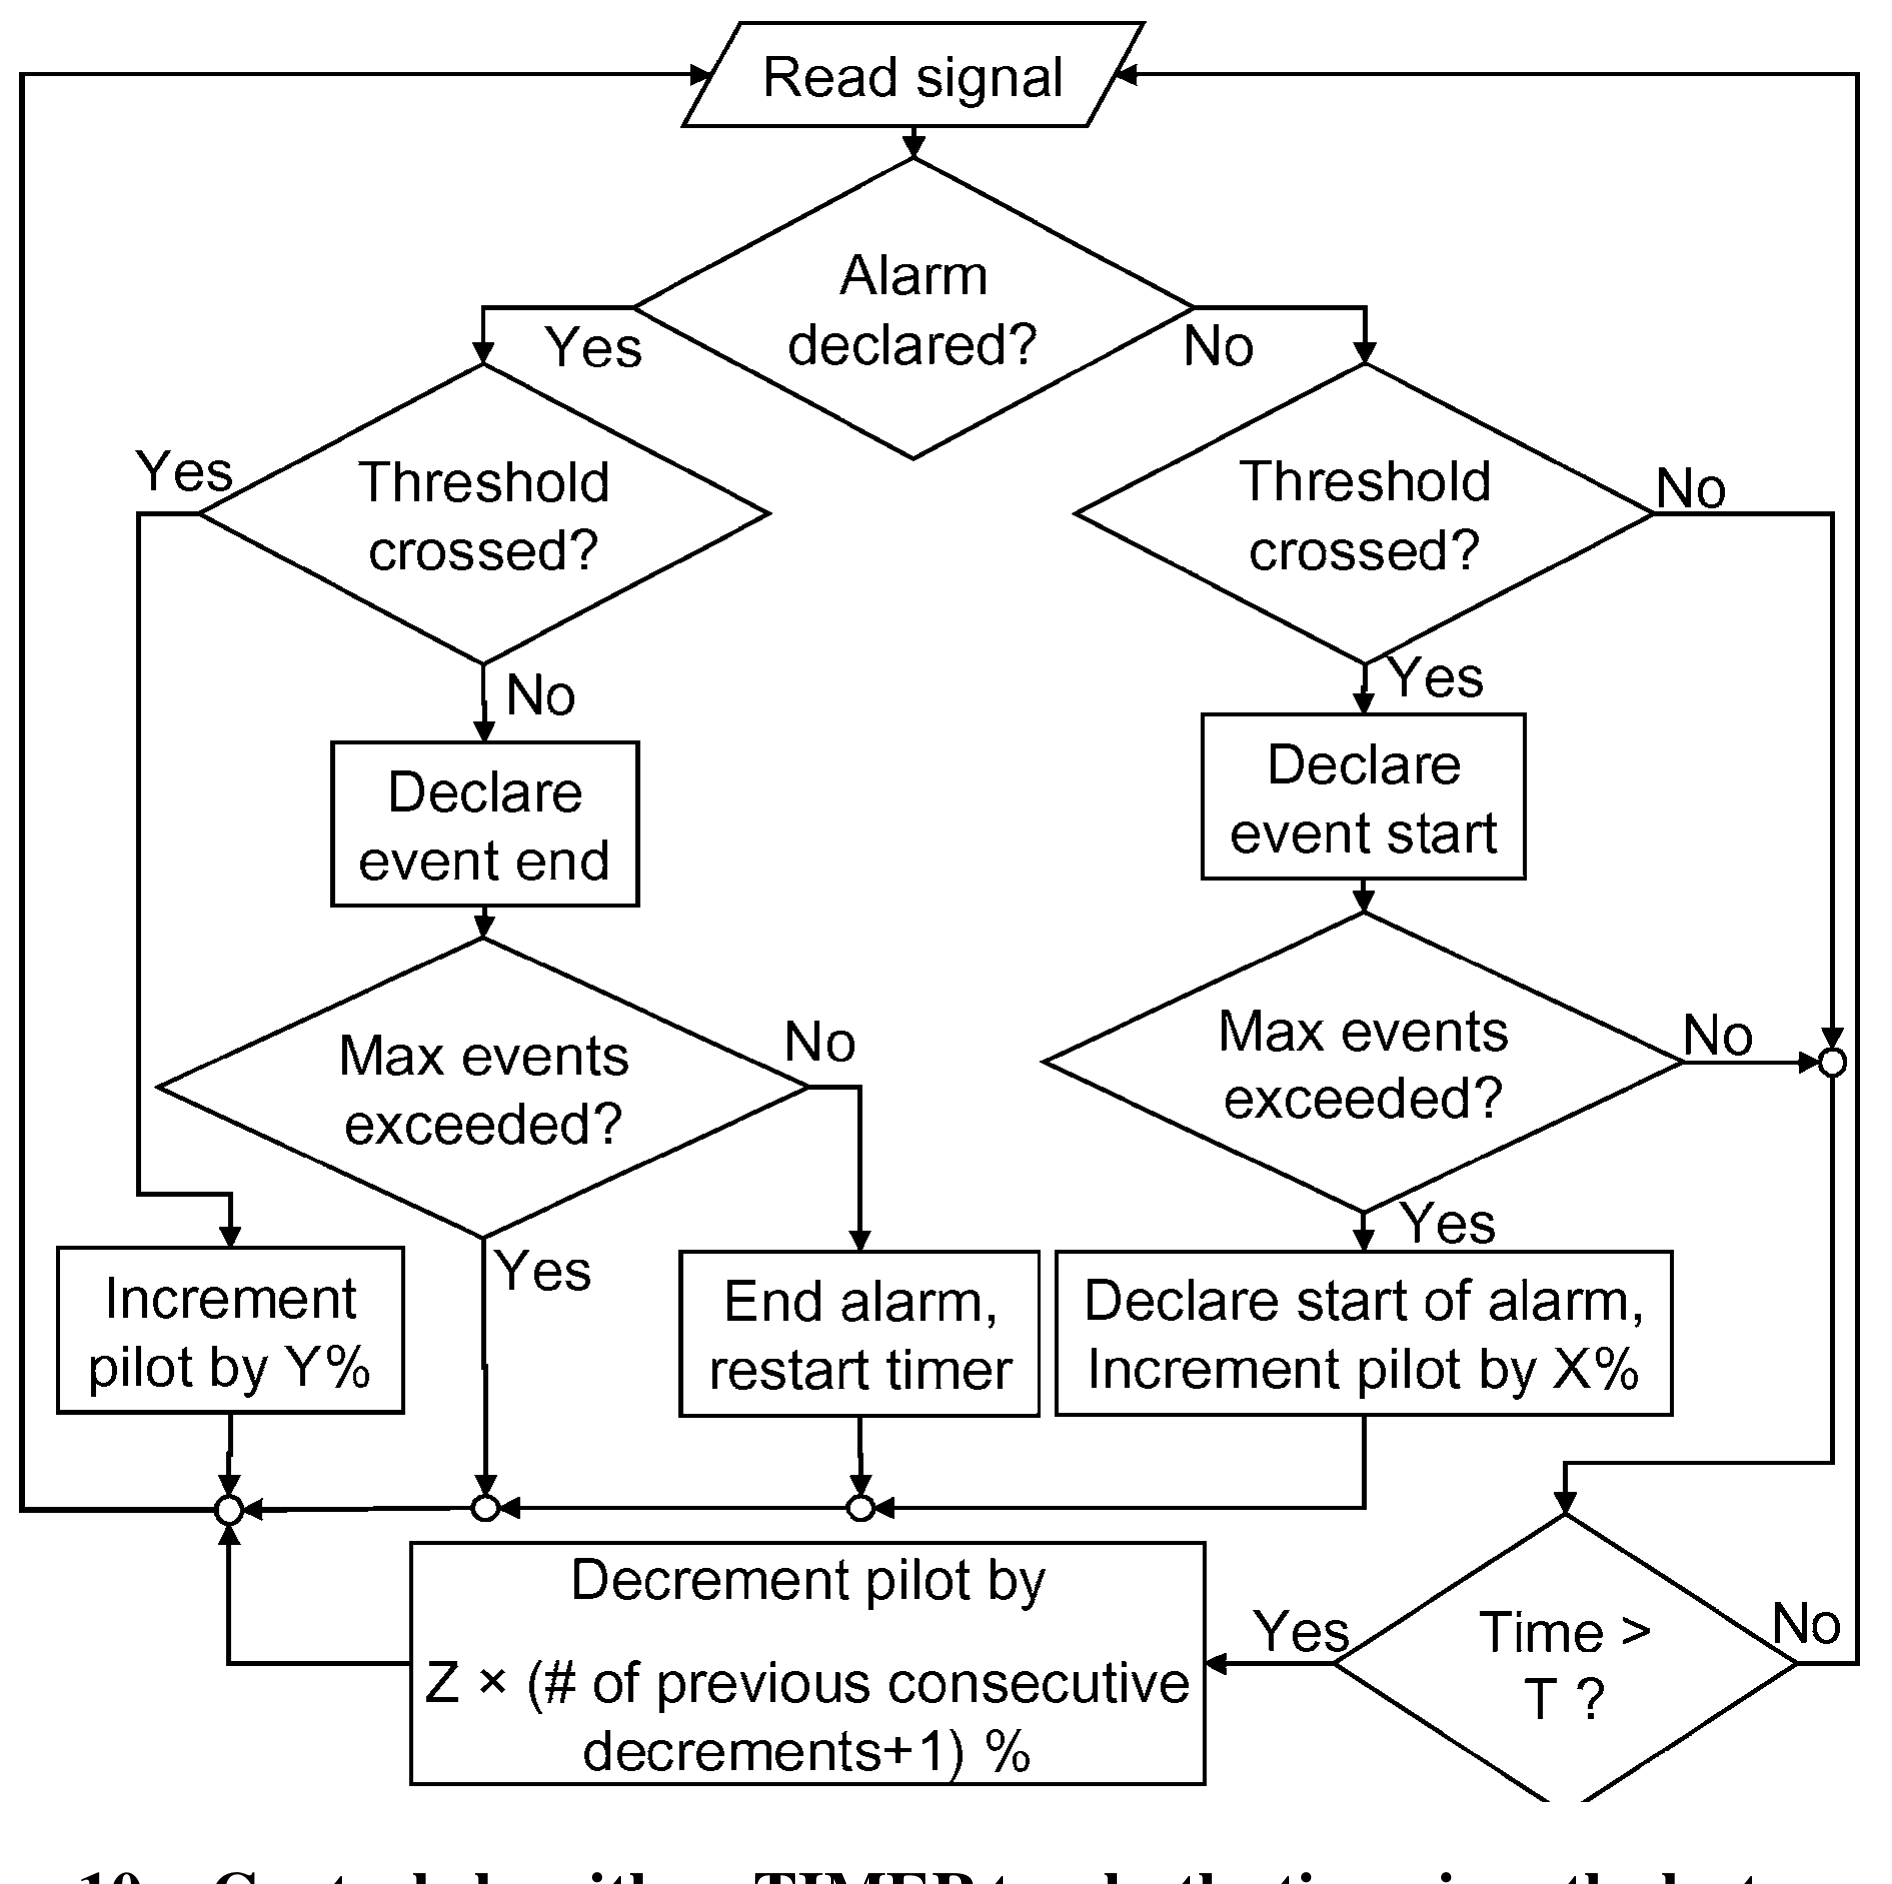
\includegraphics[width=1.000\linewidth]{figs/fig12.png}
\caption{贫油熄火主动控制的逻辑流程（引自文献[53]）}
\end{figure}
在热声不稳定性抑制方面，开环声学强迫因无需反馈传感器、系统结构简单而受到关注。Lei 等在贫预混湍流旋流火焰上把开环强迫的作用机制拆解为“自然模式抑制”与“强迫模式放大”两个并发过程，并提出了通过双频火焰响应测量先验确定有效强迫频段的控制设计框架[55]；Liao 等首次在贫预混富氢燃烧器上实验验证了开环声学强迫抑制热声振荡的有效性，指出氢体积分数 40\% 是从放大转为抑制的关键阈值[56]；Zhao 等将研究拓展至相互耦合的双振荡器系统，表明双强迫优于单强迫、且对称双强迫的能量利用效率最高[57]。

（六）现状小结

综上所述，现有研究在以下三个方面仍存在明显不足，构成本课题的切入点。

其一，反射式 TDLAS 光路的系统性研究较少，单侧接入条件下的信噪比保障与光路长期稳定性控制尚缺乏成熟方案；多光程池虽已在痕量气体检测中广泛应用[20-23]，但其与自发光高速摄影同步、同光路的融合定量测量方法尚未建立，自发光图像的定量标定仍依赖离轴或对穿式激光测量[14,26-28]。

其二，横向射流火焰的研究多集中于流动与混合过程[1-3,8]，其火焰传递函数的系统测量与多手段交叉验证数据缺乏；现有的反应横向射流强迫响应研究也未给出完整的 FTF[46]；速度脉动测量偏重多麦克风声学反演，采用热线风速仪直接测量并将其与声学反演结果交叉验证的方案尚不多见[47]。

其三，开环声学强迫抑制热声振荡的研究主要针对旋流火焰与富氢燃烧器[55-57]；基于 TDLAS 温度脉动指标的横流火焰熄火前兆判别与主动控制报道较少，该类前兆指标由旋流火焰向横流火焰的迁移能力有待进一步检验[10,51-52,54]。

\subsection{2、所阅文献的查阅范围及手段}
本课题所阅文献的时间范围主要为 1976—2026 年，同时追溯了 King（1914）关于热线对流换热规律的经典工作[58]。文献类型包括学术期刊论文、会议论文、学位论文、专著与发明专利，语言涵盖英文与中文。

文献检索手段包括：其一，以 Web of Science、Scopus、ScienceDirect、SpringerLink、Optica Publishing Group、AIP Publishing、IEEE Xplore 等外文数据库为信息源，围绕“jet in crossflow”“flame transfer function”“thermoacoustic instability”“tunable diode laser absorption spectroscopy”“multipass cell”“chemiluminescence”“lean blowout”等主题词及其组合进行检索；其二，以中国知网（CNKI）、万方数据为信息源，围绕“横向射流”“火焰传递函数”“热声不稳定”“可调谐二极管激光吸收光谱”“贫油熄火”“热线风速仪”等主题词进行检索；其三，通过已获文献的参考文献回溯与引文追踪，补全经典文献；其四，利用 Zotero 文献管理软件建立课题文献库，并对全部条目按主题、方法、年份进行归类整理，筛选出与课题直接相关的核心文献 60 篇作为重点研读对象。

\hthree{参考资料}
\vspace{0.3\baselineskip}\noindent{\bfseries 参考文献}\par
{\zihao{5}\linespread{1.25}\selectfont
\setlength{\parindent}{0pt}
\begin{enumerate}[label={[\arabic*]}, leftmargin=2.2em,
  labelsep=0.2em, itemsep=0pt, parsep=0pt, topsep=2pt, partopsep=0pt]
\item KARAGOZIAN A R. Transverse jets and their control[J]. Progress in Energy and Combustion Science, 2010, 36(5): 531-553.
\item MAHESH K. The interaction of jets with crossflow[J]. Annual Review of Fluid Mechanics, 2013, 45: 379-407.
\item ZHANG L, YANG V. Flow dynamics and mixing of a transverse jet in crossflow—Part II: Oscillating crossflow[J]. Journal of Engineering for Gas Turbines and Power, 2017, 139(8): 082602.
\item ZHANG L, YANG V. Flow dynamics and mixing of a transverse jet in crossflow—Part I: Steady crossflow[J]. Journal of Engineering for Gas Turbines and Power, 2017, 139(8): 082601.
\item CRABB D, DURÃO D F G, WHITELAW J H. A round jet normal to a crossflow[J]. Journal of Fluids Engineering, 1981, 103(1): 142-153.
\item HARRIS E W, SHOJI T, BESNARD A, et al. Effects of controlled vortex generation and interactions in transverse jets[J]. Physical Review Fluids, 2022, 7(1): 013902.
\item LI Z W, YUAN Y X, VARSEGOV V L, et al. Experimental study of the combustion characteristic of circular transverse fuel jet in crossflow[J]. Aerospace Science and Technology, 2023, 137: 108272.
\item O'CONNOR J. Visualization of shear layer dynamics in a transversely forced flow and flame[J]. Journal of Propulsion and Power, 2015, 31(4): 1127-1136.
\item GENOVA T, OTERO M, MORALES A, et al. Preheating and premixing effects on NOx emissions in a high-pressure axially staged combustor[J]. Combustion and Flame, 2022, 235: 111710.
\item MORALES A J, FORTIN M K, AHMED K A. A universal Karlovitz number to predict the lean blowoff limits of stabilized premixed flames[J]. Proceedings of the Combustion Institute, 2024, 40(1): 105312.
\item HANSON R K. Applications of quantitative laser sensors to kinetics, propulsion and practical energy systems[J]. Proceedings of the Combustion Institute, 2011, 33(1): 1-40.
\item GOLDENSTEIN C S, SPEARRIN R M, JEFFRIES J B, et al. Infrared laser-absorption sensing for combustion gases[J]. Progress in Energy and Combustion Science, 2017, 60: 132-176.
\item ALLEN M G. Diode laser absorption sensors for gas-dynamic and combustion flows[J]. Measurement Science and Technology, 1998, 9(4): 545-562.
\item LIU X, WANG G, ZHENG J, et al. Temporally resolved two dimensional temperature field of acoustically excited swirling flames measured by mid-infrared direct absorption spectroscopy[J]. Optics Express, 2018, 26(24): 31983-31994.
\item SANDERS S T, WANG J, JEFFRIES J B, et al. Diode-laser absorption sensor for line-of-sight gas temperature distributions[J]. Applied Optics, 2001, 40(24): 4404-4415.
\item MA L, CAI W, CASWELL A W, et al. Tomographic imaging of temperature and chemical species based on hyperspectral absorption spectroscopy[J]. Optics Express, 2009, 17(10): 8602-8613.
\item LIU H C, PENG F, SANDERS S T, et al. Laser absorption tomography based on unstructured meshing[J]. Measurement Science and Technology, 2023, 35(2): 025201.
\item ZHAO R, ZHOU B, ZHANG J Y, et al. A stability and spatial-resolution enhanced laser absorption spectroscopy tomographic sensor for complex combustion flame diagnosis[J]. Case Studies in Thermal Engineering, 2022, 41: 102662.
\item YANG X Y, PENG Z M, DING Y J, et al. Quantitative 2D reconstruction of temperature and OH concentration in axisymmetric flames based on ultraviolet broadband absorption tomography[J]. Combustion and Flame, 2024, 261: 113270.
\item SILVER J A. Simple dense-pattern optical multipass cells[J]. Applied Optics, 2005, 44(31): 6545-6556.
\item KASYUTICH V L, MARTIN P A. Multipass optical cell based upon two cylindrical mirrors for tunable diode laser absorption spectroscopy[J]. Applied Physics B, 2007, 88(1): 125-130.
\item ZHANG Z X, ZHOU H G, CHEN X F, et al. Design method of variable optical path length multi-pass cell[J]. Applied Physics B, 2021, 127(2): 12.
\item FENDT P, BRANDL M, PETER A, et al. Herriott cell enhanced SMF-coupled multi-scalar combustion diagnostics in a rapid compression expansion machine by supercontinuum laser absorption spectroscopy[J]. Optics Express, 2021, 29(25): 42184.
\item HARDALUPAS Y, PANOUTSOS C S, TAYLOR A M K P. Spatial resolution of a chemiluminescence sensor for local heat-release rate and equivalence ratio measurements in a model gas turbine combustor[J]. Experiments in Fluids, 2010, 49(4): 883-909.
\item MOROSHKINA A, SERESHCHENKO E, MISLAVSKII V, et al. Study of chemiluminescence of methane-air flame stabilized on a flat porous burner[J]. Combustion and Flame, 2024, 270: 113755.
\item LEE J G, SANTAVICCA D A. Experimental diagnostics for the study of combustion instabilities in lean premixed combustors[J]. Journal of Propulsion and Power, 2003, 19(5): 735-750.
\item HARDALUPAS Y, ORAIN M. Local measurements of the time-dependent heat release rate and equivalence ratio using chemiluminescent emission from a flame[J]. Combustion and Flame, 2004, 139(3): 188-207.
\item ECKBRETH A C. Laser diagnostics for combustion temperature and species[M]. 2nd ed. Amsterdam: Gordon and Breach Publishers, 1996.
\item 反射式 TDLAS 与 PIV/PLIF 同时拍摄装置: 中国, CN121252888A[P]. 2026.
\item DUCRUIX S, SCHULLER T, DUROX D, et al. Combustion dynamics and instabilities: Elementary coupling and driving mechanisms[J]. Journal of Propulsion and Power, 2003, 19(5): 722-734.
\item SCHULLER T, DUROX D, CANDEL S. A unified model for the prediction of laminar flame transfer functions: comparisons between conical and V-flame dynamics[J]. Combustion and Flame, 2003, 134(1-2): 21-34.
\item CANDEL S. Combustion dynamics and control: Progress and challenges[J]. Proceedings of the Combustion Institute, 2002, 29(1): 1-28.
\item CANDEL S, DUROX D, SCHULLER T, et al. Progress and challenges in swirling flame dynamics[J]. Comptes Rendus Mécanique, 2012, 340(11-12): 758-768.
\item CANDEL S, DUROX D, SCHULLER T, et al. Dynamics of swirling flames[J]. Annual Review of Fluid Mechanics, 2014, 46: 147-173.
\item PALIES P, DUROX D, SCHULLER T, et al. Dynamics of premixed confined swirling flames[J]. Comptes Rendus Mécanique, 2009, 337(6-7): 395-405.
\item PALIES P, DUROX D, SCHULLER T, et al. The combined dynamics of swirler and turbulent premixed swirling flames[J]. Combustion and Flame, 2010, 157(9): 1698-1717.
\item BAILLY C, DUROX D, JUNIPER M, et al. A dedicated paper for Pr Sébastien Candel EM2C laboratory, CentraleSupélec[J]. Combustion and Flame, 2025, 279: 114301.
\item WANG K, LAERA D, YANG D. Thermoacoustic limit cycle prediction and acoustic dissipation rate quantification for annular combustors using a 2D wave-based low-order network model[J]. Combustion and Flame, 2026, 291: 115142.
\item POINSOT T. Prediction and control of combustion instabilities in real engines[J]. Proceedings of the Combustion Institute, 2017, 36(1): 1-28.
\item LIEUWEN T C. Unsteady combustor physics[M]. Cambridge: Cambridge University Press, 2012.
\item DOWLING A P, MAHMOUDI Y. Combustion noise[J]. Proceedings of the Combustion Institute, 2015, 35(1): 65-100.
\item JI C Z, SHI W T, KE E L, et al. Characterization of the nonlinear responses of swirling flames in a premixed gas turbine combustor with varying bluff-body blocking ratios under acoustic forcing[J]. Aerospace Science and Technology, 2026, 176: 112207.
\item DHARMAPUTRA B, NAGPURE P, IMPAGNATIELLO M, et al. Flame transfer function measurement of a sequential combustor fuelled with natural gas and hydrogen[J]. Combustion and Flame, 2025, 274: 113972.
\item 张金锋, 胡宏斌, 姜磊, 等. 氢混燃料旋流预混火焰传递函数的实验研究[J]. 推进技术, 2025, 46(1): 2311007.
\item 王子豫, 朱彤. 燃气燃烧热声不稳定研究进展[J]. 洁净煤技术, 2026, 32(5): 1-15.
\item CHOI Y, HAN G, KIM K T. Forced response of transverse reacting jet in vitiated crossflow to harmonic velocity disturbances[J]. Combustion and Flame, 2024, 269: 113670.
\item VISHNYAKOV O I, POLIVANOV P A, SIDORENKO A A. Comparison of hot-wire and particle image velocimetry measurements in the zone of interaction of a shock wave with a boundary layer at Mach number of 1.43[J]. Physics of Fluids, 2021, 33(11): 111704.
\item MCMANUS K R, POINSOT T, CANDEL S M. A review of active control of combustion instabilities[J]. Progress in Energy and Combustion Science, 1993, 19(1): 1-29.
\item DOCQUIER N, BELHADJ M, LACAS F. Combustion control and sensors: a review[J]. Progress in Energy and Combustion Science, 2002, 28(2): 107-150.
\item NAIR S, LIEUWEN T. Acoustic detection of blowout in premixed flames[J]. Journal of Propulsion and Power, 2005, 21(1): 32-39.
\item YI T X, GUTMARK E J. Real-time prediction of incipient lean blowout in gas turbine combustors[J]. AIAA Journal, 2007, 45(7): 1734-1739.
\item ZHANG B, LIU H Y, LIU X C, et al. Prediction method of swirling flame lean blowout based on flame image morphological features[J]. Applied Sciences, 2023, 13(5): 3173.
\item MURUGANANDAM T M, NAIR S, SCARBOROUGH D, et al. Active control of lean blowout for turbine engine combustors[J]. Journal of Propulsion and Power, 2005, 21(5): 807-814.
\item LI H, ZHOU X, JEFFRIES J B, et al. Active control of lean blowout in a swirl-stabilized combustor using a tunable diode laser[J]. Proceedings of the Combustion Institute, 2007, 31(2): 3215-3223.
\item LEI Y, LIAO Y, ZHANG J, et al. Mitigation of thermoacoustic oscillations by open-loop acoustic forcing: Physical mechanisms and an a priori control-design framework[J]. Combustion and Flame, 2026, 289: 115014.
\item LIAO Y, CHOI Y, LIU P, et al. Active control of thermoacoustic instability in a lean-premixed hydrogen-enriched combustor via open-loop acoustic forcing[J]. Combustion and Flame, 2025, 277: 114175.
\item ZHAO C, ZHENG L, ZHOU J, et al. Dynamics of two mutually coupled thermoacoustic oscillators under external dual forcing[J]. Nonlinear Dynamics, 2025, 113(22): 31039-31061.
\item KING L V. On the convection of heat from small cylinders in a stream of fluid: Determination of the convection constants of small platinum wires with applications to hot-wire anemometry[J]. Philosophical Transactions of the Royal Society A, 1914, 214: 373-432.
\item BRUUN H H. Hot-wire anemometry: principles and signal analysis[M]. Oxford: Oxford University Press, 1995.
\item COMTE-BELLOT G. Hot-wire anemometry[J]. Annual Review of Fluid Mechanics, 1976, 8: 209-231.
\end{enumerate}
}
\vspace{0.5\baselineskip}
\section{三、研究内容、技术路线、创新点}
\subsection{1、主要研究内容及拟解决的关键技术}
\subsubsection{（1）主要研究内容}
1）反射式 TDLAS 测量系统研制与方法建立。设计并搭建反射式 TDLAS 光路，包括 2 $\mu$m 分布反馈（distributed feedback，DFB）激光器、自主设计的反射镜架与高透玻璃窗口、螺纹光学支架固定方案；完成出光调试与信号采集；建立吸收光谱基线拟合、Voigt 线型拟合与温度/柱浓度反演的数据处理流程。计划选用 H\textsubscript{2}O 在 2 $\mu$m 附近的一对低态能级差较大的吸收线实施双线测温，其中高波数线作为低温线、低波数线作为高温线，通过两条谱线积分吸收面积之比反演路径平均温度，同时由积分吸收面积反演 H\textsubscript{2}O 柱浓度。

2）反射式 TDLAS 与自发光高速摄影融合测量。实现 TDLAS 与自发光高速摄影的同步、同光路采集；以 TDLAS 定量反演的温度与柱浓度为基准，建立自发光图像强度与热化学参数之间的映射关系；结合 301 项目提供的伺服电机扫描系统获取二维温度场，获得横流火焰温度场与结构的同步定量表征。

3）横流火焰传递函数测量。研制课题组自研恒温式热线风速仪（CTA，钨丝探头）直接测量声激励下的速度脉动；采用 SiPM 光电探测器配合 CH*/OH* 窄带滤光片测量热释放率脉动；采用压力传感器配合半无限长管测量压力脉动；在单频步进扫频声激励下进行多参数同步采集，获得速度$\rightarrow$热释放、速度$\rightarrow$压力、速度$\rightarrow$CH* 自发光的多组频域传递函数（幅值与相位），并进行多方法交叉验证。

4）基于 TDLAS 温度脉动指标的熄火主动控制。尝试将 FFT\%[0-50] 熄火前兆指标迁移至横流火焰，利用 2 $\mu$m TDLAS 测得的 H\textsubscript{2}O 吸收线温度波动构建熄火前兆判据；设计以声激励或流量调节为执行手段的闭环主动控制实验，评估控制开启前后火焰位置、温度脉动与自发光强度的变化，考察其对火焰位置与稳定性的调控效果。

5）横流火焰热声不稳定性的组织与机理研究。在贫预混条件下调整出口收缩段与带孔板的孔径，使声波在上下游之间形成较强反射，诱导横流火焰产生自激热声振荡；测量其共振频率与声学模态，结合相位平均图像判别主导耦合量（火焰面积、火焰高度或当量比脉动），为传递函数测量提供与自激工况一致的物理参照。

\subsubsection{（2）拟解决的关键技术}
1）反射式光路的信噪比与长期稳定性保障。反射光程设计、杂散光抑制（镜架与光学支架发黑处理、窗口选型）与光路漂移控制；在单侧接入条件下，需解决反射光斑回偏导致的光强波动与基线漂移问题，采用参考光路与基线自校正算法抑制漂移。

2）多传感器同步测量的时序一致性。TDLAS、自发光高速摄影、CTA、SiPM 与压力传感器由同一时钟源统一触发，并对各通道进行时序标定，以提高多参数在同一激励周期内的相位一致性；相位偏差宜控制在激励周期的 1\% 以内，否则将影响 FTF 相位的准确性。

3）自研 CTA 的频响与标定。基于热平衡原理与 \mbox{King's} 定律标定曲线（$E^{2}$ = A + $B\cdot U^{n}$）建立输出电压与流速的定量关系，通过最小二乘拟合确定 A、B、n 三个标定常数；需解决闭环电桥电路的稳定性与带宽验证问题，并评估探头污染与温度漂移对测量结果的影响。

4）横流火焰 FTF 的可靠提取。激励频率分辨率与步长选择（拟采用 20—500 Hz、步长 10 Hz 的单频步进扫频）、采样率拟取最高激励频率的 10 倍以上、信噪比较弱频段的辨识、以及热线风速仪直接测量与双麦克风声学反演结果的一致性判据。

5）横流火焰自激振荡的激发与工况边界。出口收缩度与带孔板孔径直接决定声反射强度与共振频率，需确定可稳定激发自激热声振荡的几何与运行参数，避免工况落入无声反馈的稳定区；同时需解决自激振荡与扫频强迫两种工况之间的一致性验证问题。

\subsection{2、拟采取的研究方法、技术路线、实施方案及可行性分析}
\subsubsection{（1）研究方法}
1）理论分析与数值模拟方法。采用 SolidWorks 完成横流燃烧试验台与反射式镜架的三维建模，采用 FLUENT 对试验段冷态流场进行数值模拟，分析横流来流与横向射流的速度场分布、回流区范围与出口收缩段对声学边界条件的影响，为结构参数与测点位置选取提供依据。

2）光谱仿真方法。基于 HITRAN 高分辨率分子吸收光谱数据库，结合辐射传输模型与谱线计算，仿真 H\textsubscript{2}O 在 2 $\mu$m 波段不同温度、不同波长下的吸收光谱，筛选吸收强度适中、彼此邻近且不受其他组分干扰的一对吸收线，用于双线测温。

3）激光吸收光谱测量方法。采用 DAS 与 WMS 相结合的方式：以 DAS 扫描获取完整吸收线型用于温度与浓度反演，以 WMS 配合锁相解调获取信噪比较高的脉动信号，用于熄火前兆判别。

4）多参数同步实验方法。由同一时钟源统一触发激光扫描、高速相机、CTA、SiPM 与压力传感器，在扫频声激励下同步采集各通道信号，通过互谱或锁相方法提取频域传递函数。

5）数据处理与反演方法。TDLAS 数据经基线拟合与 Voigt 线型拟合后按双线法反演温度与柱浓度；自发光图像经预处理、火焰边缘提取与强度归一化后按振荡周期进行相位平均；FTF 由激励信号作为相位参考通过互谱方法提取。

\subsubsection{（2）技术路线与实施方案}
本课题按“平台建设—测量方法建立—响应规律测量—主动控制验证”四个阶段推进，总体技术路线如图 13 所示。实验系统由横流燃烧试验台、反射式 TDLAS 测量光路、自发光高速摄影与化学发光测量系统、速度与压力脉动测量系统、同步触发与数据采集系统五部分组成，试验台总体布局如图 14 所示。其中，横流燃烧试验台以空气为横流来流、甲烷/氢气为燃料，采用敞开式供气与集成化电源布置，出口设置可更换的收缩段与带孔板用于调节声学边界条件；反射式 TDLAS 测量光路选用 2 $\mu$m DFB 激光器，激光经准直后穿过试验段高透玻璃窗口入射至火焰区，由自主设计的反射镜架将光束折返，使发射与接收单元集成于试验台同一侧；自发光高速摄影配合 CH*（430 nm）与 OH*（310 nm）窄带滤光片，与 TDLAS 同光路、同步采集火焰自发辐射图像，SiPM 光电探测器则用于测量火焰全局化学发光强度；速度脉动由课题组自研恒温式热线风速仪直接测量，压力脉动由压力传感器配合半无限长管测量；各通道由同一时钟源统一触发并完成时序标定，以保证多参数在同一激励周期内的相位一致性。

\begin{figure}[H]
\centering
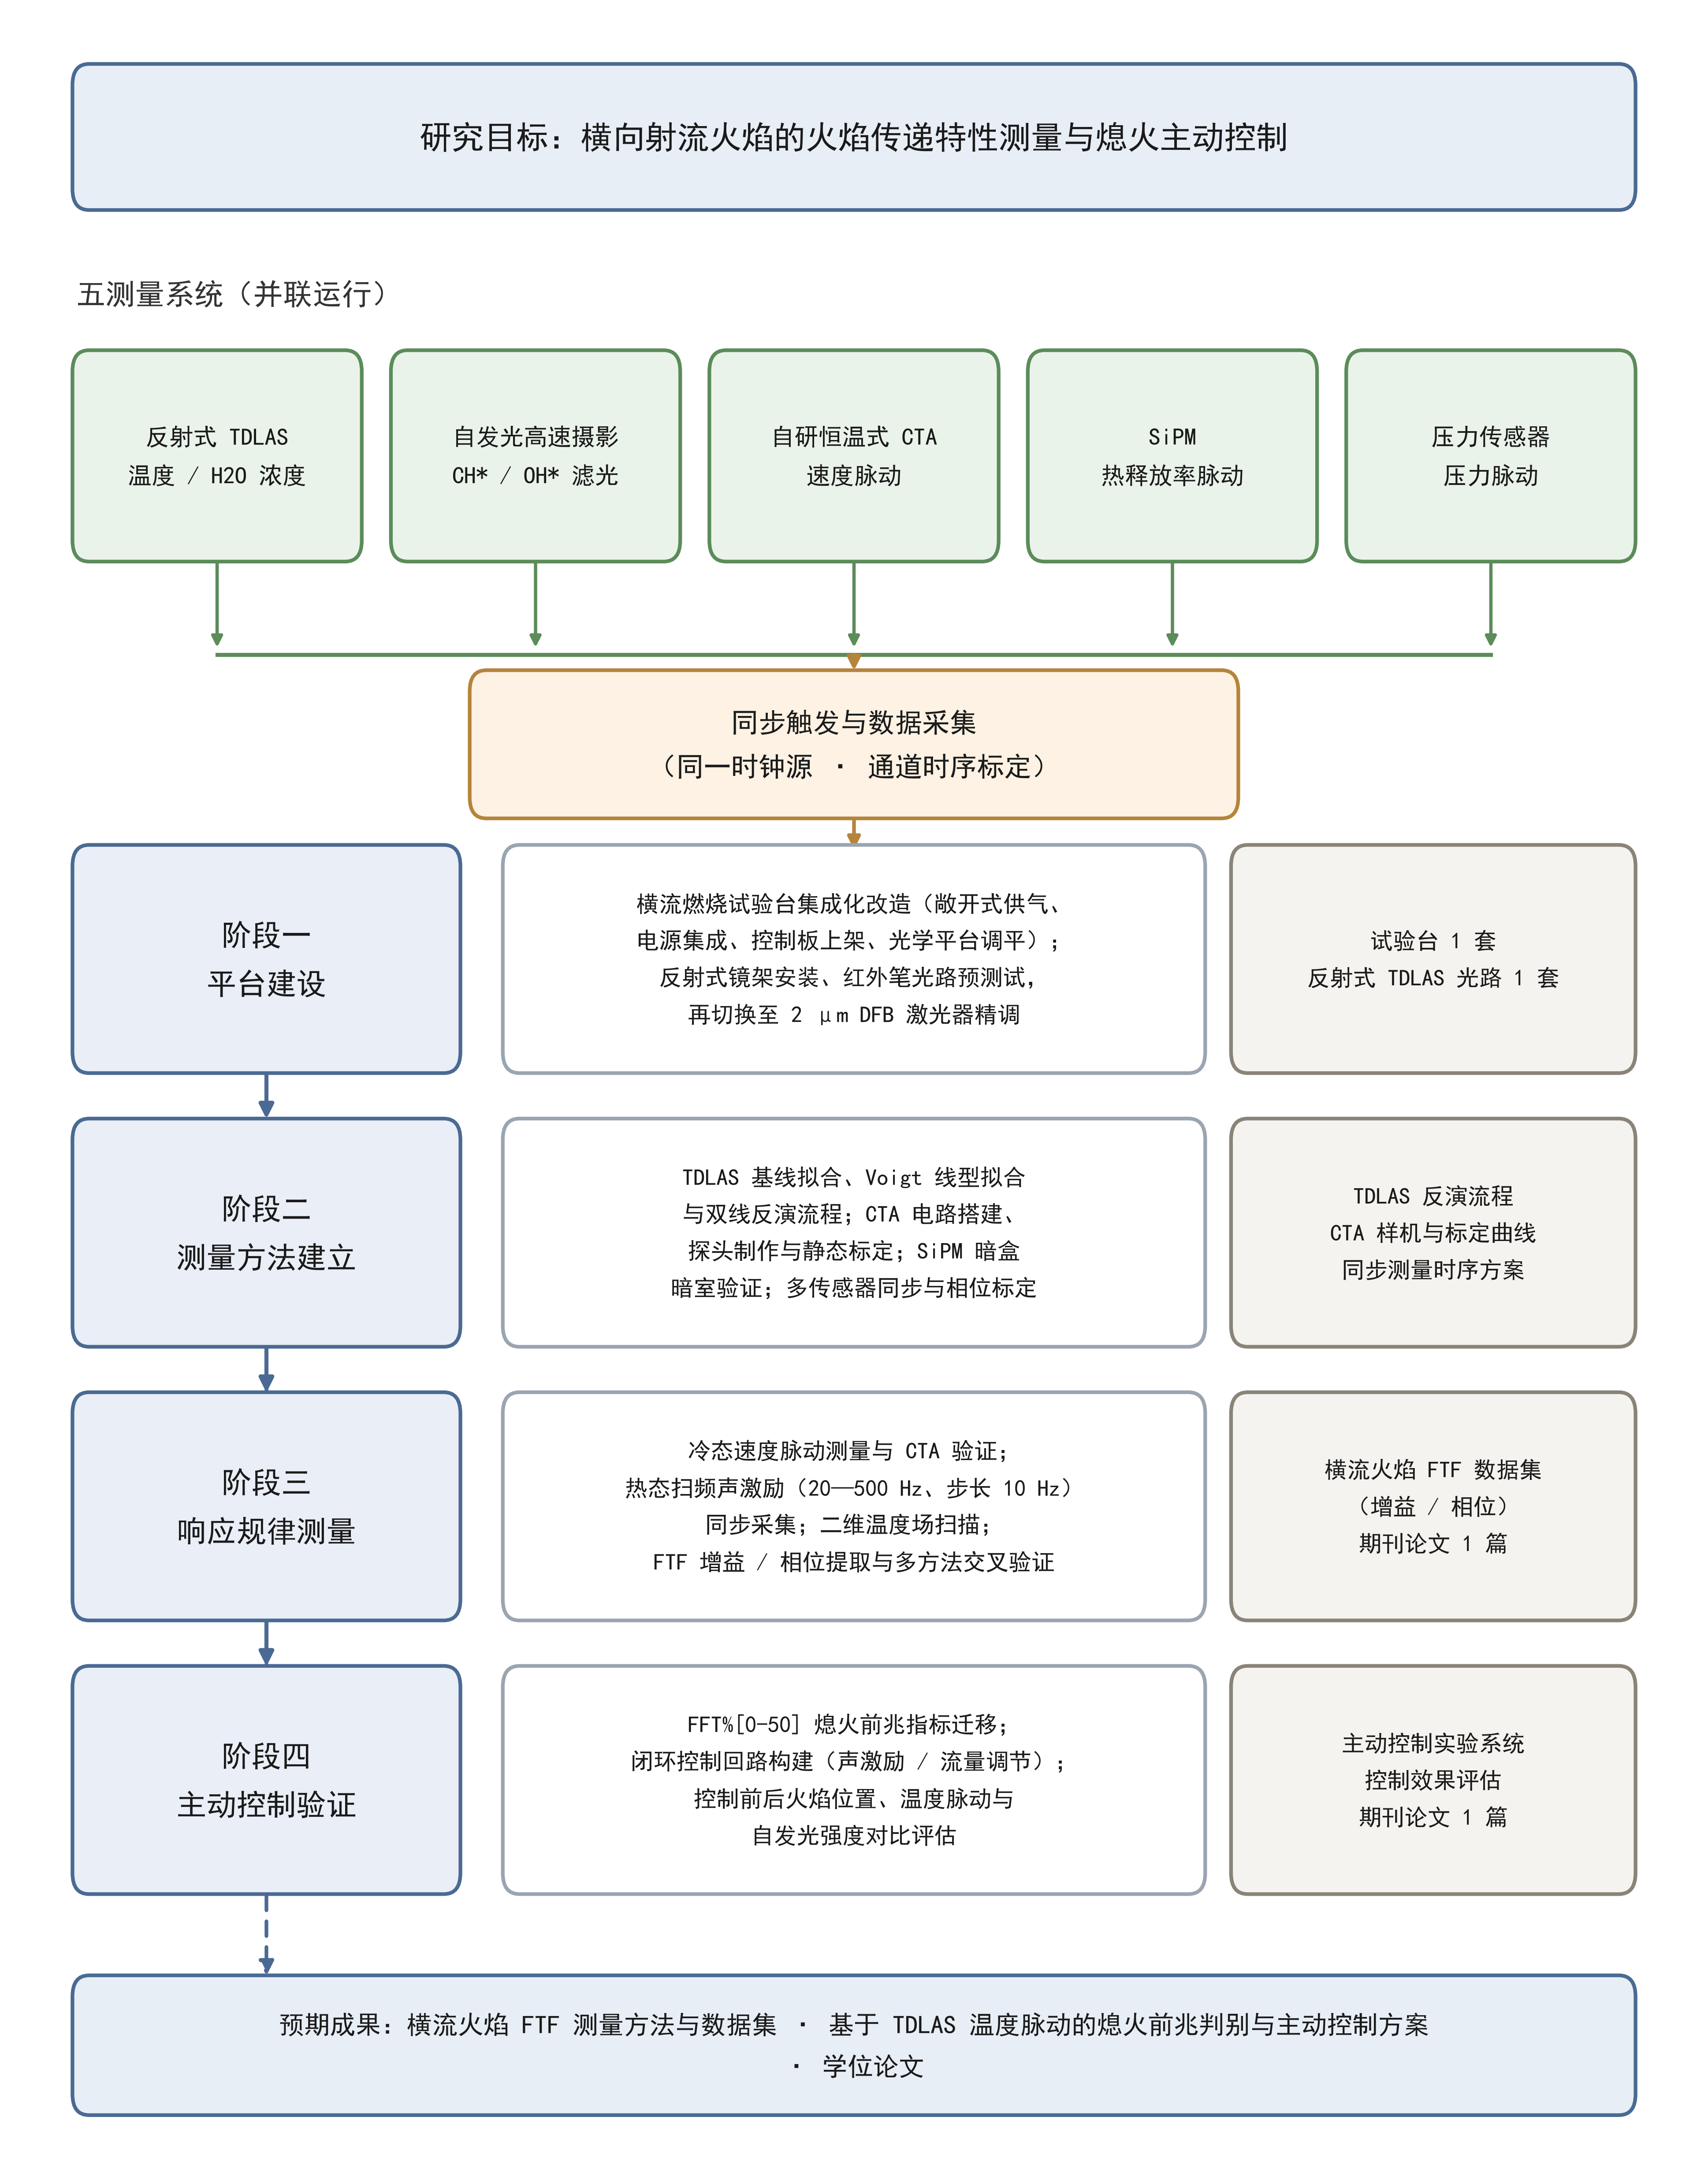
\includegraphics[width=0.795\linewidth]{figs/fig13.png}
\caption{本课题技术路线（四阶段主线与五测量系统并联）}
\end{figure}
1）平台建设阶段。完成横流燃烧试验台集成化改造：供气系统采用敞开式设计，电源集成化布置，气体控制板上架，面包板光学平台调平；完成反射式 TDLAS 镜架的安装与光路预测试，先以红外笔/红光验证光路布局，再切换至 2 $\mu$m DFB 激光器精细调节。

2）测量方法建立阶段。完成反射式 TDLAS 出光与温度/柱浓度反演流程；完成自研 CTA 电路搭建与探头制作并完成静态标定；完成反射式光路预测试与出光调试；开展 SiPM 暗盒的暗室功能验证；建立多传感器同步触发方案。

3）响应规律测量阶段。开展冷态速度脉动测量与 CTA 验证；开展热态扫频声激励实验，同步采集 TDLAS 温度、自发光图像、CTA 速度、SiPM 热释放率与压力信号；结合 301 项目提供的伺服电机扫描系统获取二维温度场；反演并提取 FTF，并与双麦克风声学反演结果交叉验证。

4）主动控制验证阶段。基于 TDLAS 温度脉动计算熄火前兆指标，构建闭环控制回路，开展主动控制实验并评估控制效果；整理数据，完成学位论文撰写。

\begin{figure}[H]
\centering
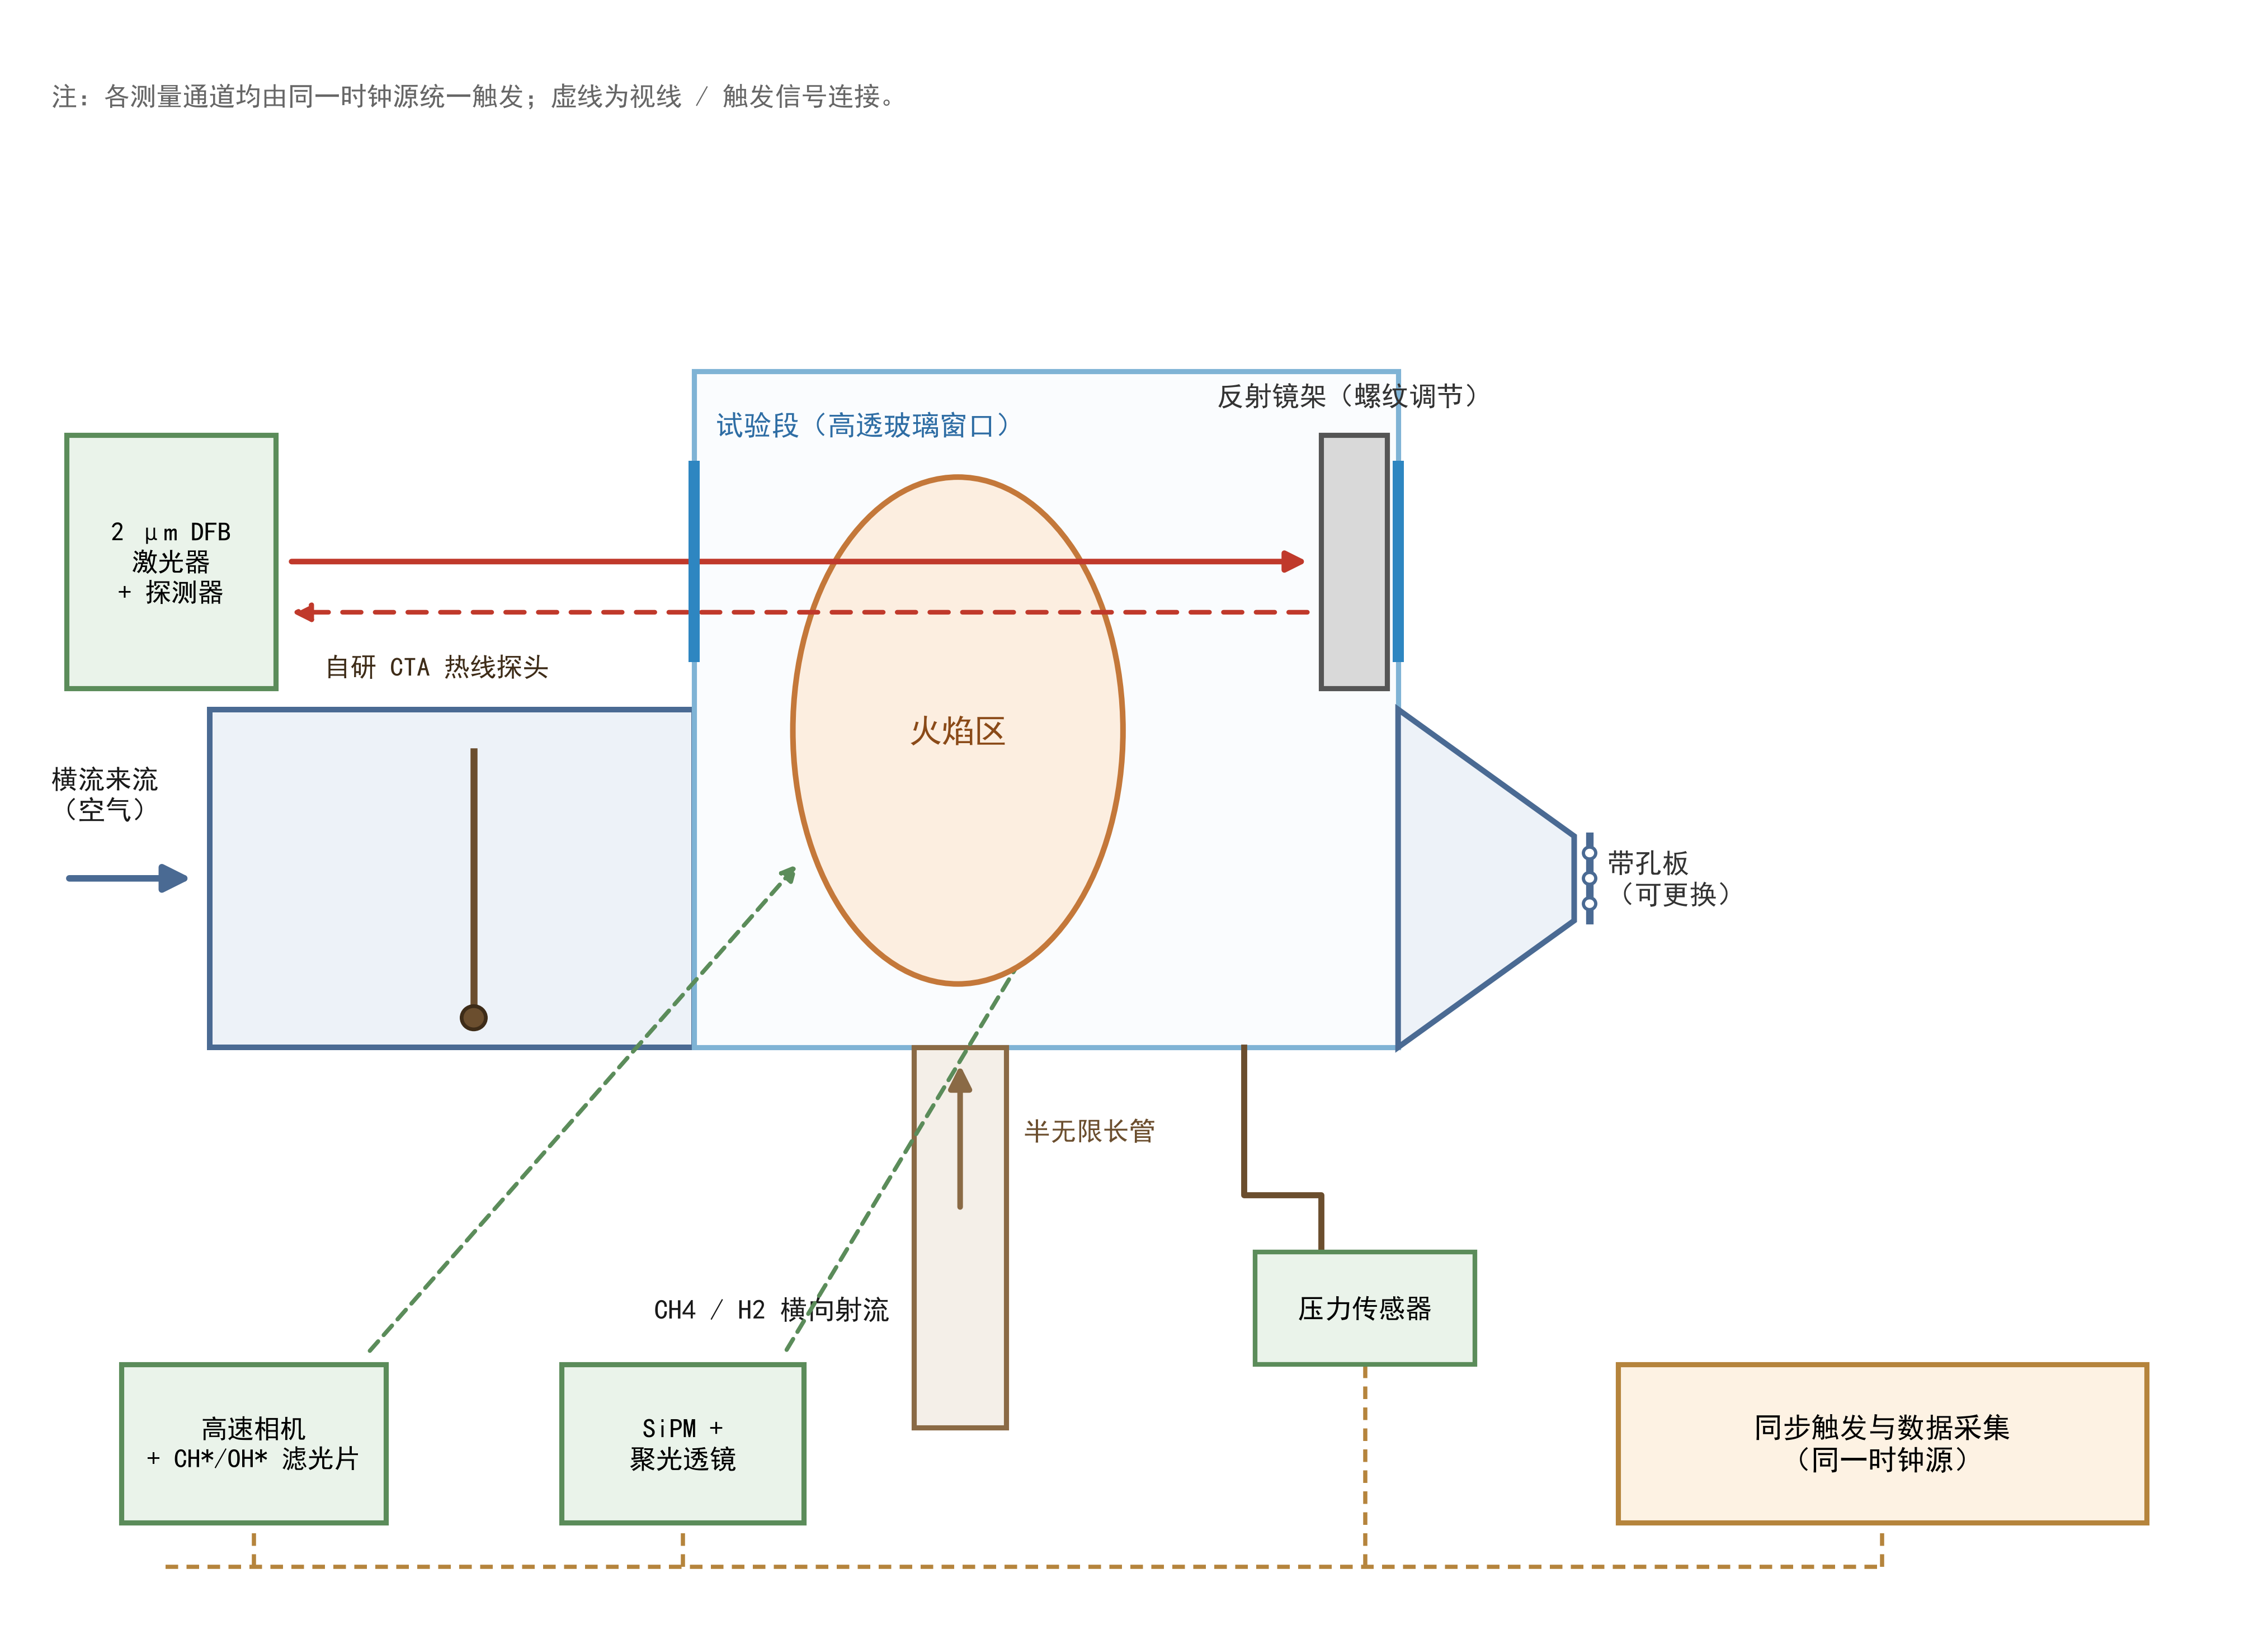
\includegraphics[width=0.991\linewidth]{figs/fig14.png}
\caption{试验台总体布局示意（横流燃烧试验台与多参数同步测量系统）}
\end{figure}
作为方法参照，图 15 与图 16 分别给出了旋流燃烧实验系统的组成与声激励条件下火焰传递函数测量试验台的布置[42-43]，其测量链路的组织方式可为本文试验台的搭建提供参考。

\begin{figure}[H]
\centering
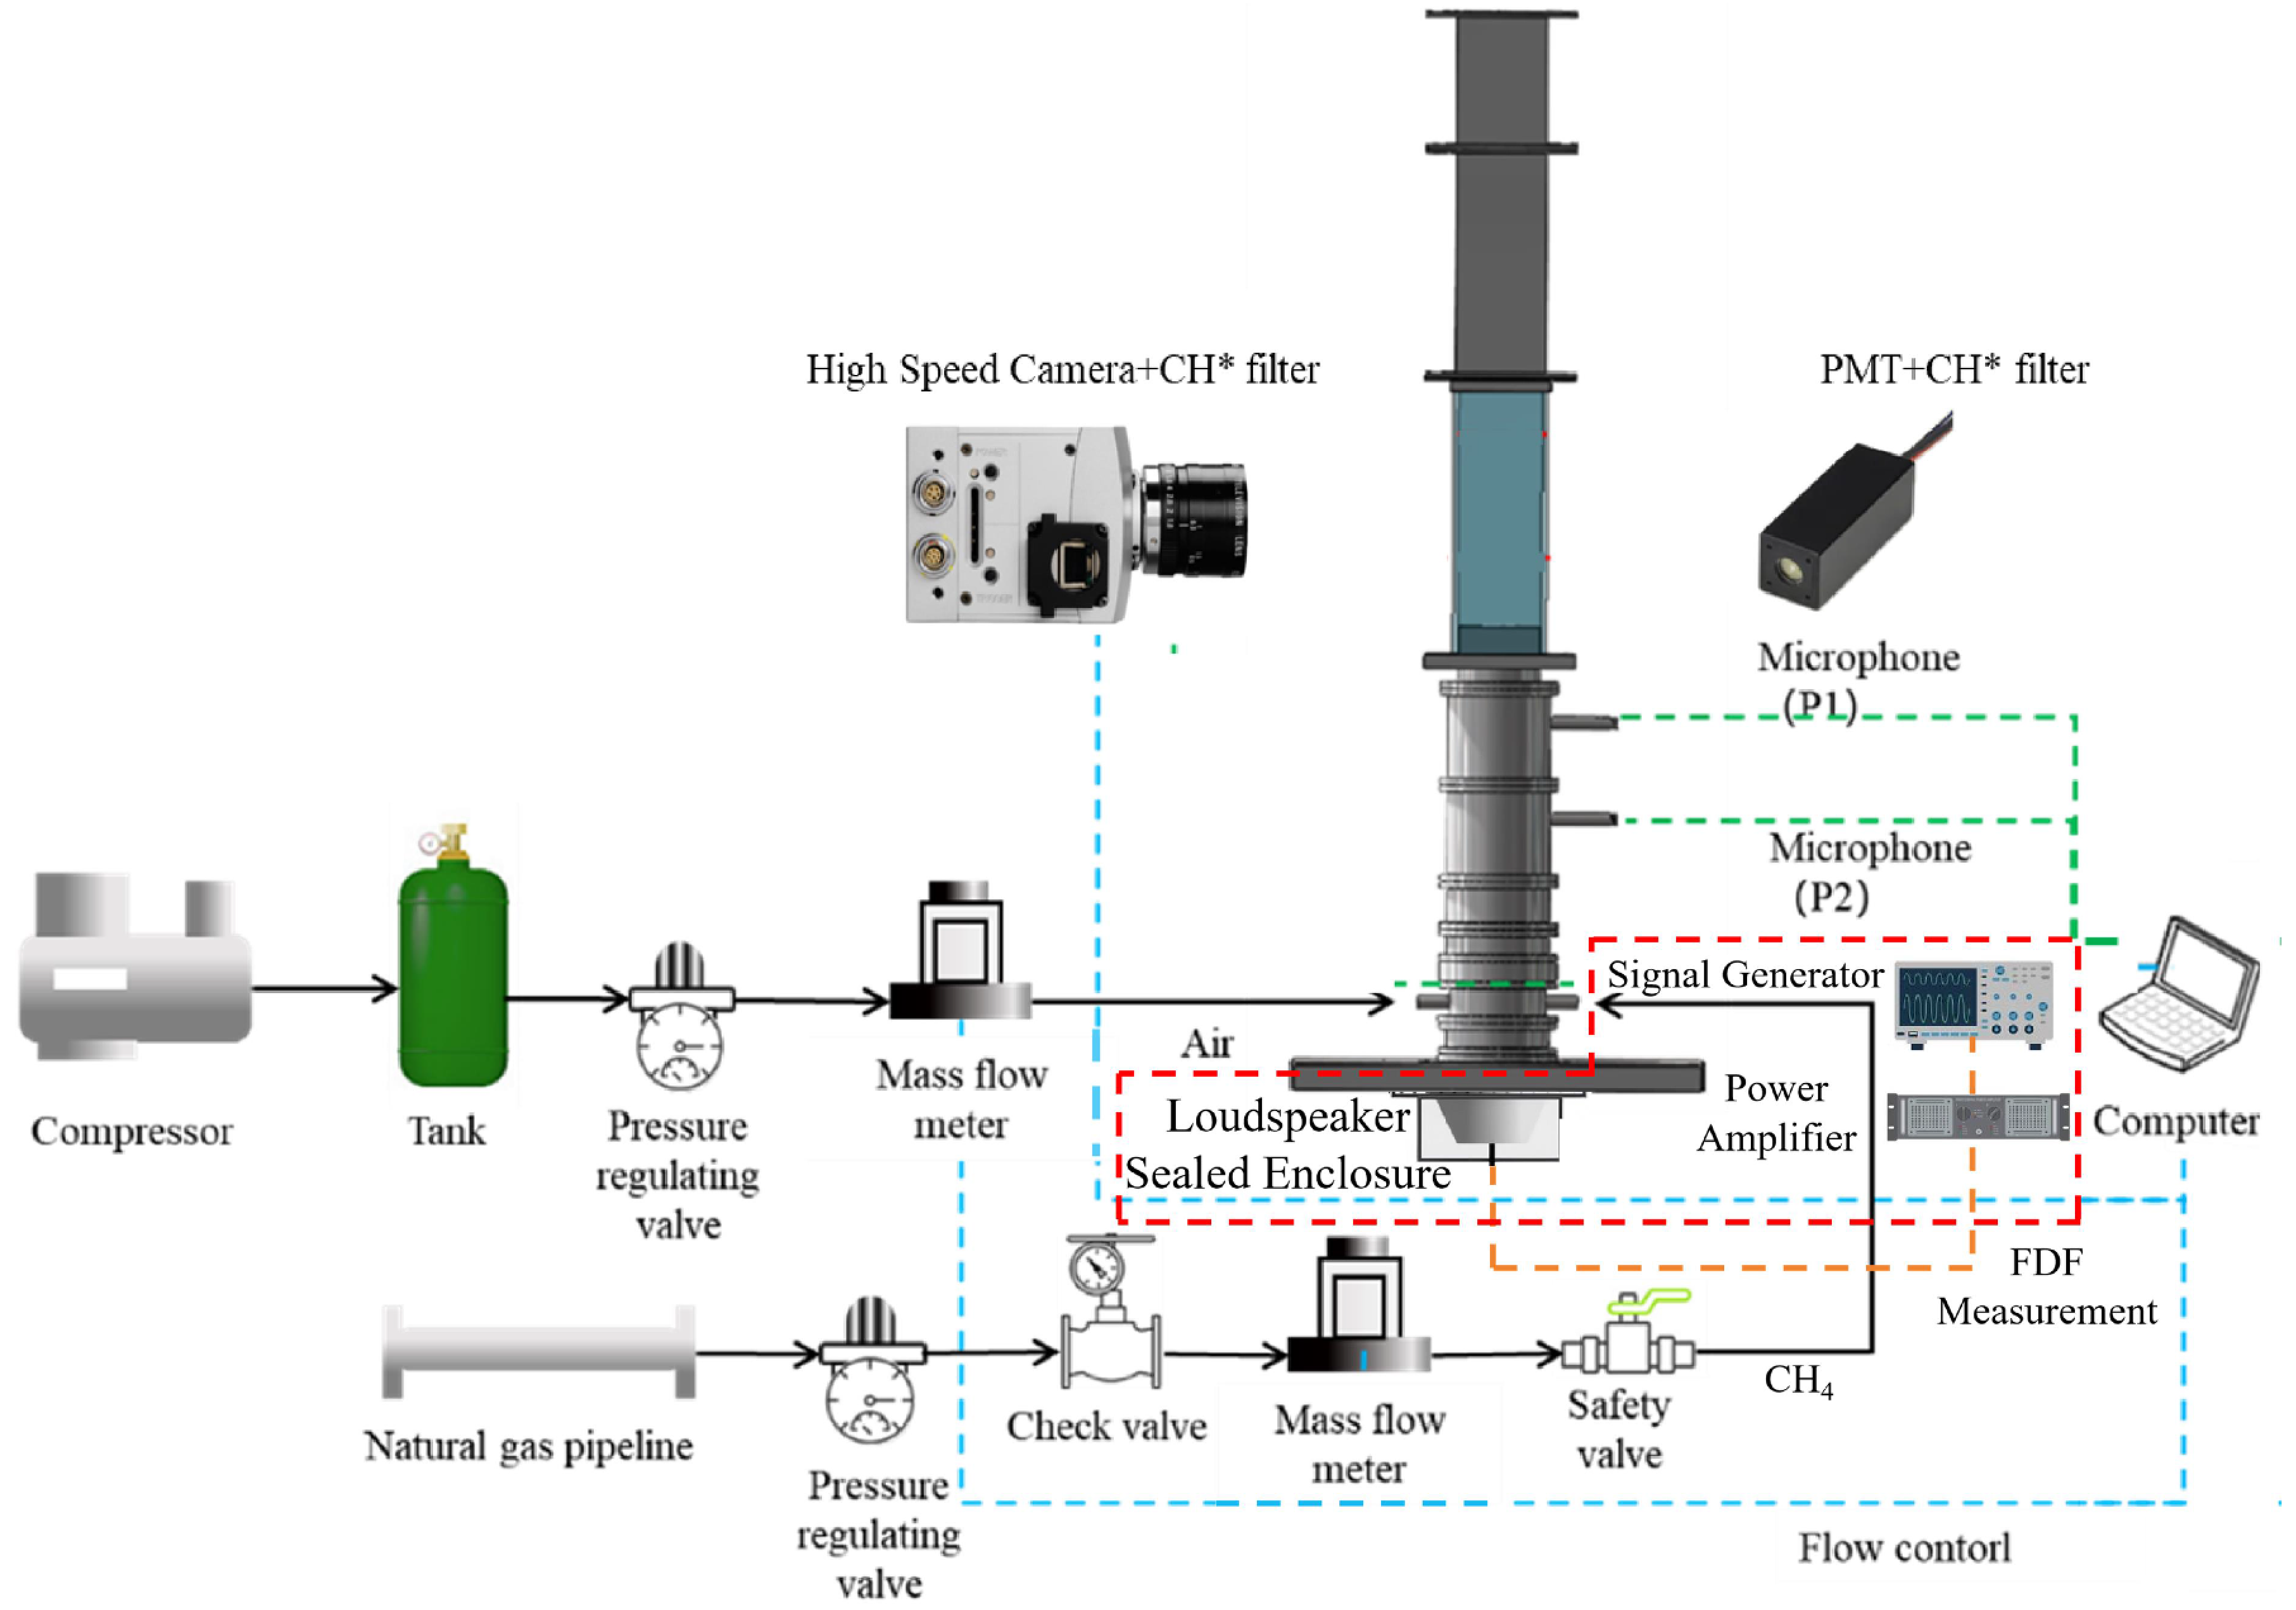
\includegraphics[width=1.000\linewidth]{figs/fig15.png}
\caption{旋流燃烧实验系统组成示意（供气、激励与测量单元）（引自文献[42]）}
\end{figure}
\begin{figure}[H]
\centering
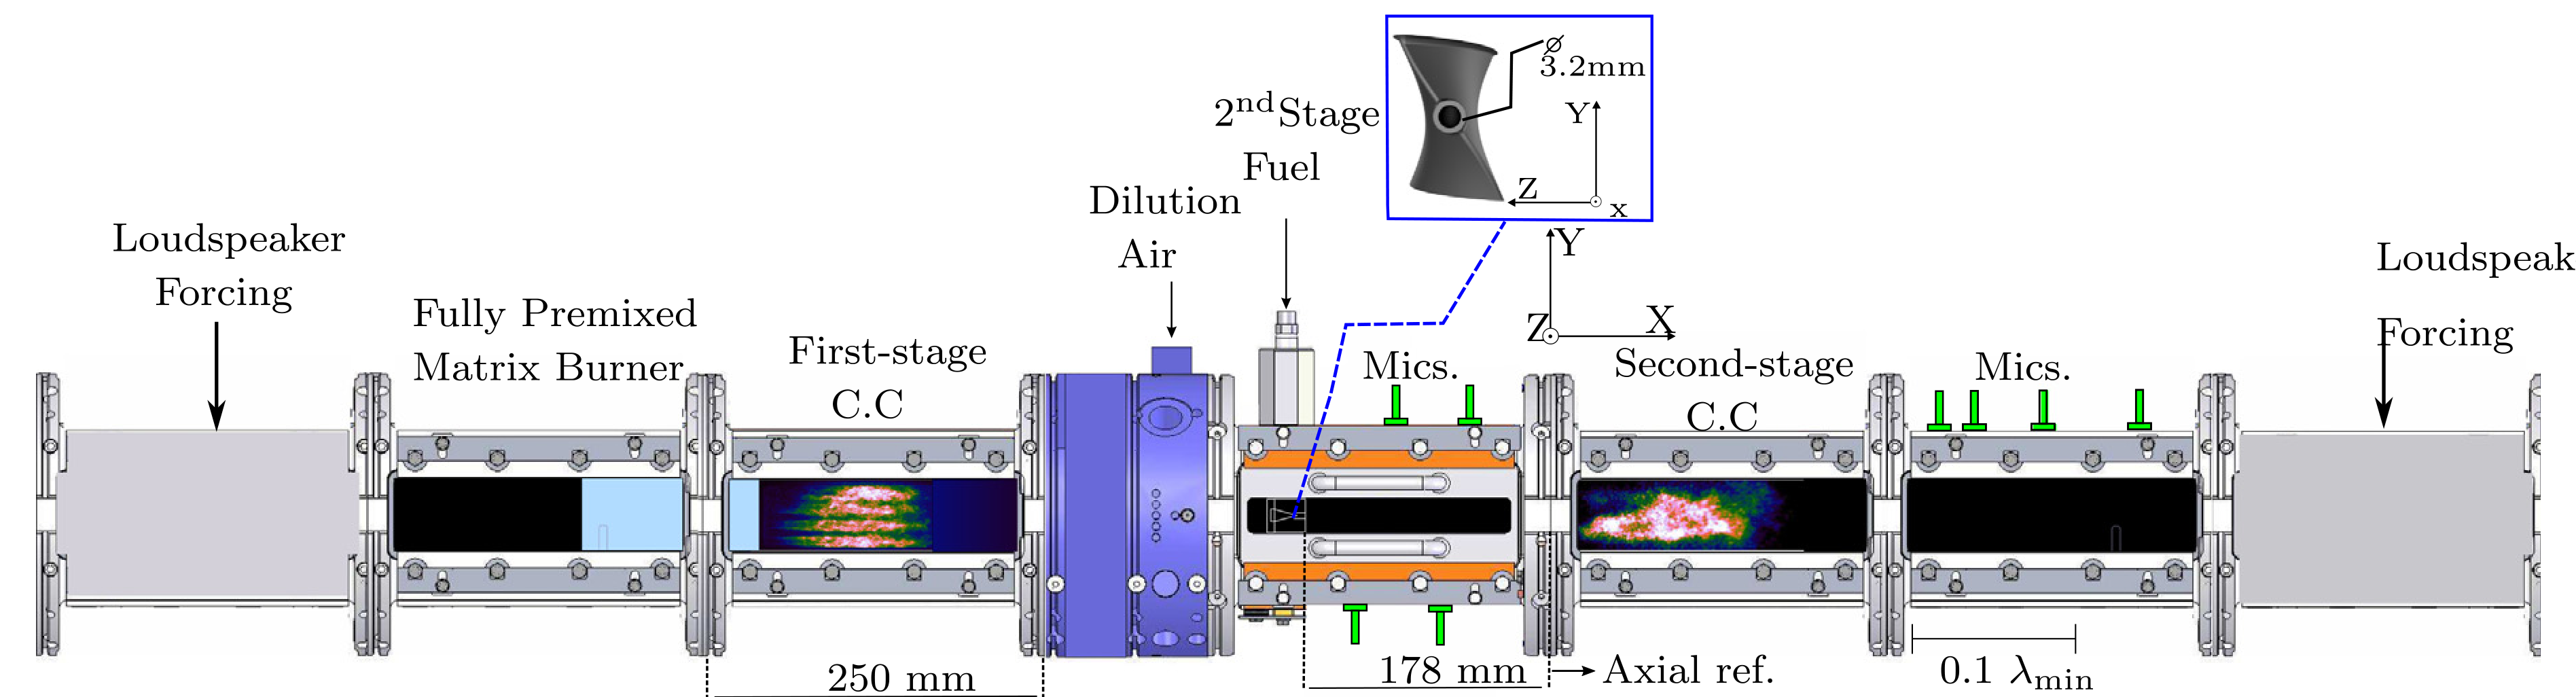
\includegraphics[width=1.000\linewidth]{figs/fig16.png}
\caption{声激励火焰传递函数测量试验台（引自文献[43]）}
\end{figure}
\subsubsection{（3）可行性分析}
1）理论与技术可行。一方面，横向射流的流动结构、掺混特性与声强迫响应已有较为系统的研究积累[1-2,6,8]，多光程/腔增强光路的设计方法亦较为成熟[20,22-23]，本课题的技术方案在此基础上提出，具有较好的理论基础。另一方面，反射式 TDLAS 采用双线法测温，其选线原则、Voigt 线型拟合方法与温度反演流程均有可借鉴的成熟范式[11-12,14,16]；FTF 的扫频测量与互谱提取方法也有 Dharmaputra 等[43]的框架可以参照。

2）实验条件可行。硬件条件方面，课题组的横流燃烧试验台供气系统、电源系统与光学平台已基本搭建完成；反射式镜架已完成加工、验收、发黑处理与螺纹光学支架安装，高透玻璃窗口已就位待固定；SiPM 暗盒已完成组装、尚待暗室功能验证；自研 CTA 已完成理论设计、LTspice 直流工作点仿真验证与首根探头样品制作，电路搭建正在进行；2 $\mu$m DFB 激光器与课题组 215 项目共用，使用时间窗口尚在协调中。软件条件方面，课题组配有 SolidWorks、FLUENT、LTspice 等仿真软件与 HITRAN 光谱数据库，具备开展结构建模、流场仿真与光谱仿真计算的条件。

3）风险与对策。其一，CTA 首次搭板存在反馈极性错误与自激振荡风险，已通过 LTspice 仿真预审并请导师审阅电路图，实验中将采用逐级上电与示波器观测的方式排查；其二，2 $\mu$m DFB 激光器为课题组与 215 项目共用设备，存在时间窗口冲突风险，将通过协调使用时间窗口、必要时交叉使用、并对关键实验提前预约机时予以控制；其三，反射式镜架与出口收缩段等结构件需外协加工，存在进度风险，将通过定期催办与提前下单予以控制；其四，自激热声振荡的激发条件较为敏感，若在既定几何参数下无法稳定激发，将退而采用外部声强迫工况开展 FTF 测量，并以强迫工况结果作为主动控制的依据。

\subsection{3、论文的创新点}
1）测量方法探索。在横流燃烧平台上尝试建立反射式 TDLAS 与自发光高速摄影同步、同光路的融合测量方法：仅需单侧光学通道即可完成激光发射与接收，以 TDLAS 定量反演的温度与柱浓度为基准，探索自发光图像的定量化，兼顾定量精度与二维结构分辨，以期缓解传统对穿式光路在空间受限平台上难以布置的问题[15,21,29]。目前已自主完成反射式镜架的设计、加工、发黑处理与螺纹光学支架装配，高透玻璃窗口已验收就位，为光路搭建提供了硬件基础。

2）测量对象与手段拓展。拟系统测量横向射流火焰的火焰传递函数，尝试补充横流火焰动力学响应数据；采用课题组自研恒温式热线风速仪直接测量速度脉动、以之与多麦克风声学反演结果相互对照，并以 SiPM 热释放率脉动与压力脉动测量实现多手段交叉验证[5,47,58-60]。目前自研 CTA 已完成理论设计、LTspice 直流工作点仿真与首根钨丝探头样品制作（冷态电阻 8—9 $\Omega$），电路搭建正在进行。

3）应用拓展。尝试将基于 TDLAS 温度脉动的 FFT\%[0-50] 熄火前兆指标由旋流火焰迁移至横向射流火焰，探索以声激励或流量调节为执行手段的闭环主动控制方案并开展实验验证，检验该类前兆指标在横流火焰上的工况适应性与可迁移性[51-52,54]。目前已完成 2 $\mu$m 波段 H2O 双线测温谱线对的筛选与 FFT\%[0-50] 指标计算流程的梳理。

\section{四、研究基础}
\subsection{1、所需实验手段、研究条件和实验条件}
\subsubsection{（1）实验手段}
本课题以实验研究为主、光谱仿真为辅。光谱仿真方面，基于 HITRAN 数据库仿真 H\textsubscript{2}O 在 2 $\mu$m 波段的吸收光谱，筛选测温谱线对并评估温度灵敏度。实验方面，采用反射式 TDLAS 双线法反演路径平均温度与 H\textsubscript{2}O 柱浓度；采用自发光高速摄影配合 CH*/OH* 窄带滤光片获取火焰二维结构与热释放率脉动；采用自研恒温式热线风速仪直接测量速度脉动；采用 SiPM 光电探测器配合滤光片测量全局化学发光强度；采用压力传感器配合半无限长管测量压力脉动；由同一时钟源统一触发各通道实现多参数同步采集，并以声激励系统施加扫频扰动，最终提取横流火焰的传递函数并构建熄火主动控制回路。

\subsubsection{（2）研究和实验条件}
课题组具备开展本课题所需的场地与实验设施：横流燃烧试验台（含供气系统、流量控制与安全保护装置）已完成集成化改造；拥有 2 $\mu$m 分布反馈激光器、光电探测器、高性能数据采集卡与光学平台，基本具备开展 TDLAS 与自发光成像实验的条件；具有多波长的光学镜片、光学支架与聚光抛物面镜，可自行搭建设计反射式光路；拥有高性能计算机，可进行流场仿真与光谱仿真计算；实验室水冷机、气源与排风系统基本齐备，能够满足长时间点火与热态实验的安全要求。此外，课题组在燃烧不稳定性诊断、激光吸收光谱测量与多参数同步测量方面具有一定的前期工作积累与实验流程，可为本课题提供技术支持。

\subsection{2、所需经费，包含经费来源、开支预算}
\subsubsection{（1）经费来源}
导师项目科研经费。

\subsubsection{（2）开支预算}
\begin{table}[H]
\centering
\zihao{5}
\caption{开支预算}
\setlength{\tabcolsep}{4pt}
\begin{tabular}{l r p{8.6cm}}
\toprule
名称 & 金额/元 & 备注 \\
\midrule
工控机 & 12000 & 研华 IPC-610L 工业控制计算机 \\
试验台加工 & 26000 & 横流燃烧试验台集成化改造与结构件外协加工 \\
铝型材 & 1200 & 欧标 40$\times$40 铝型材，用于平台框架搭建 \\
可调平台 & 1600 & 可调角度光学平台，调节范围 3$^{\circ}$，重复精度 0.01 mm \\
伺服电机 & 6800 & 二维扫描用伺服电机及驱动器，行程 35 cm \\
光路器件 & 8600 & 镜片、光学支架、聚光抛物面镜、反射镜架 \\
激光器 & 16000 & 2 $\mu$m 分布反馈（DFB）激光器及驱动电源 \\
光电探测器 & 9800 & 700—2200 nm 光电探测器 2 只、SiPM 光电探测器 \\
流量计 & 11000 & 甲烷/氢气/空气专用电控质量流量计 \\
减压阀 & 2400 & 高压气瓶专用减压阀 \\
气管 & 600 & 不锈钢及聚四氟乙烯气路管件 \\
水冷机 & 3600 & 冷却水循环机，容量 12 L、扬程 2 m \\
耗材 & 8000 & 实验用气体、钨丝、滤光片、电子元器件等 \\
\midrule
合计 & 107600 &  \\
\bottomrule
\end{tabular}
\end{table}
\vspace{0.4\baselineskip}
\subsection{3、前期工作基础}
（1）横流燃烧试验台集成化改造进展。已完成横流燃烧试验台的集成化改造：供气系统改为敞开式设计，燃料与氧化剂管路重新敷设并加装阻火器与单向阀；电源系统由分散布置改为集中集成化布置，减小了对光学测量的电磁干扰；气体控制板上架固定，便于操作与读数；面包板光学平台完成调平，为反射式光路与高速相机提供了稳定的安装基准。改造后的试验台可满足横流来流速度、燃料射流流量与出口声学边界条件的联合调节需求。

（2）反射式 TDLAS 镜架与光路调试进展。已完成反射镜架的概念设计、图纸迭代、铜套方案定型、外协加工与到货验收，镜架尺寸与表面处理合格，铜套与精密调节螺钉配合顺滑；镜架金属件已完成发黑处理以抑制杂散光，并安装螺纹固定光学支架替代原磁力底座（铝制面包板不导磁、磁力方案不可行），镜架固定方案基本解决。试验段高透玻璃窗口（125$\times$125 mm）已验收合格并已就位，待实验前固定。光路拟采用“先红外笔/红光预测试、后 2 $\mu$m DFB 激光器精调”的两步调试流程，尚待试验台安装到位后启动光路预测试与出光调试。

（3）自研恒温式热线风速仪进展。已完成理论设计：以热平衡原理为基础，建立输出电压 E 与流速 U 之间的 \mbox{King's} 定律关系 $E^{2}$ = A + $B\cdot U^{n}$，并据此设计闭环恒温电桥电路；已完成 LTspice 直流工作点仿真，验证了各支路工作点与桥路平衡条件，仿真结果已请导师审阅；已完成首根钨丝探头样品制作，室温下冷态电阻实测为 8—9 $\Omega$，在预期范围内，验证了机械压接工艺的电气连接可靠性；探头静态标定的实验方案与数据处理脚本已准备就绪。

（4）探测器件与光源准备进展。SiPM 光电探测器暗盒已完成打孔组装，电源板侧盖安装、评估板螺丝固定、BNC 线缆干涉问题均已解决，暗盒遮光与结构稳固性检查良好，尚待开展暗室功能验证，以确认无饱和、信噪比可接受，为全局化学发光强度的低噪声测量提供条件；2 $\mu$m DFB 激光器与课题组 215 项目共用，需协调使用时间窗口，目前尚在协调中，无需另行购置。

（5）前期成果。课题组已提交发明专利《反射式 TDLAS 与 PIV/PLIF 同时拍摄装置》（课题组惠昊主笔），为本课题的融合测量方法提供了知识产权与硬件方案基础；本课题的小论文大纲已经确认，明确了“测量方法—响应规律—主动控制”的研究主线与三篇论文的选题分工。

（6）定量结果与预研数据。在光谱仿真方面，已开展 2 $\mu$m 波段 H\textsubscript{2}O 吸收线的筛选计算，初步确定以约 7153.75 cm\textsuperscript{$-1$} 与 7154.35 cm\textsuperscript{$-1$} 附近的一对吸收线作为候选测温谱线对，两条线的低态能级差在 1000—2500 K 温度区间内具有可用的温度灵敏度，仿真得到的双线积分吸收比随温度单调变化，在 1500 K 附近相对灵敏度约为 1.5\%/100 K。在测量方案方面，拟采用扫频范围 20—500 Hz、步长 10 Hz，采样率拟取最高激励频率的 10 倍以上（即不低于 5 kHz）。在 CTA 方面，已完成电桥参数初步设计，预期带宽约 10 kHz 量级，标定拟采用标准射流喷嘴在 0.5—30 m/s 速度范围内取若干工况点进行最小二乘拟合。

\section{五、工作计划}
\begin{table}[H]
\centering
\zihao{5}
\caption{工作计划}
\setlength{\tabcolsep}{2pt}
\begin{tabular}{p{0.9cm} p{4.3cm} p{2.1cm} p{3.1cm} p{3.1cm}}
\toprule
序号 & 阶段及内容 & 工作量\newline（时数） & 起讫日期 & 阶段成果形式 \\
\midrule
1 & 文献调研与开题：完成开题报告与文献综述 & 240 & 2026.09—2026.10 & 开题报告、文献综述 \\
2 & 横流燃烧试验台集成化改造与反射式 TDLAS 光路搭建调试 & 320 & 2026.10—2026.12 & 试验台一套、反射式 TDLAS 光路一套 \\
3 & 自研恒温式热线风速仪电路搭建、探头制作与静态标定 & 280 & 2026.11—2027.02 & CTA 样机及 \mbox{King's} 定律标定曲线 \\
4 & 多传感器同步测量方案建立与冷态/热态预实验 & 300 & 2027.02—2027.04 & 同步测量时序方案、预实验数据集 \\
5 & 扫频声激励下横流火焰 FTF 测量与多方法交叉验证 & 520 & 2027.04—2027.08 & 横流火焰 FTF 数据集、期刊论文 1 篇 \\
6 & 基于 TDLAS 温度脉动的熄火前兆判别与闭环主动控制实验 & 480 & 2027.08—2027.12 & 主动控制实验系统及控制效果评估、期刊论文 1 篇 \\
7 & 学位论文撰写与答辩准备 & 360 & 2028.01—2028.05 & 学位论文《基于反射式 TDLAS 与多参数同步测量的横向射流火焰传递特性及主动控制实验研究》、答辩 \\
\midrule
合计 & — & 2500 & — & — \\
\bottomrule
\end{tabular}
\end{table}
\vspace{0.4\baselineskip}
\clearpage
\section{六、评审意见}
\begin{center}{\zihao{4}\bfseries 山东科技大学硕士研究生学位论文开题报告评分表}\end{center}
\begin{center}
\renewcommand{\arraystretch}{1.5}
\begin{tabular}{|c|c|c|c|}
\hline
\textbf{评审项目} & \textbf{分值} & \textbf{评分标准} & \textbf{得分（百分制）} \\
\hline
\multirow[t]{3}{*}{一、选题依据} & \multirow[t]{3}{*}{30 分} & 21\textasciitilde{}30 分 & \\ \hline
 & & 11\textasciitilde{}20 分 & \\ \hline
 & & 0\textasciitilde{}10 分 & \\ \hline
\multirow[t]{3}{*}{二、理论基础
和专门知识} & \multirow[t]{3}{*}{20 分} & 15\textasciitilde{}20 分 & \\ \hline
 & & 6\textasciitilde{}15 分 & \\ \hline
 & & 5 分以下 & \\ \hline
\multirow[t]{3}{*}{三、选题难度
及先进性} & \multirow[t]{3}{*}{30 分} & 21\textasciitilde{}30 分 & \\ \hline
 & & 11\textasciitilde{}20 分 & \\ \hline
 & & 0\textasciitilde{}10 分 & \\ \hline
\multirow[t]{3}{*}{四、文字表达} & \multirow[t]{3}{*}{10 分} & 8\textasciitilde{}10 分 & \\ \hline
 & & 4\textasciitilde{}7 分 & \\ \hline
 & & 3 分以下 & \\ \hline
\multirow[t]{3}{*}{五、口头报告} & \multirow[t]{3}{*}{10 分} & 8\textasciitilde{}10 分 & \\ \hline
 & & 3\textasciitilde{}7 分 & \\ \hline
 & & 3 分以下 & \\ \hline
\textbf{总分} & & & \\ \hline
\end{tabular}
\end{center}
\vspace{0.4\baselineskip}
\vspace{0.6\baselineskip}\noindent{\bfseries 开题评审小组组成：}\par
\renewcommand{\arraystretch}{2.0}
\noindent\begin{tabularx}{\textwidth}{|>{\centering\arraybackslash}p{1.6cm}|>{\centering\arraybackslash}p{2.4cm}|>{\centering\arraybackslash}p{2.4cm}|X|>{\centering\arraybackslash}p{2.6cm}|}
\hline
\textbf{组成} & \textbf{姓名} & \textbf{职称} & \textbf{单位} & \textbf{签字} \\ \hline
导师 &  &  &  &  \\ \hline
组长 &  &  &  &  \\ \hline
成员 &  &  &  &  \\ \hline
成员 &  &  &  &  \\ \hline
成员 &  &  &  &  \\ \hline
\end{tabularx}
\vspace{0.4\baselineskip}
\noindent\hfill 年\hspace{1.2cm}月\hspace{1.2cm}日\hspace{0.6cm}\par
\vspace{0.4\baselineskip}
\noindent\fbox{\parbox{\dimexpr\textwidth-2\fboxsep-2\fboxrule\relax}{%
\vspace{0.3cm}
\textbf{导师对本课题的评价}\par
\vspace{4.4cm}
\noindent\hfill 导师签名\hfill 年\hspace{1.1cm}月\hspace{1.1cm}日\hspace{0.3cm}\par
\vspace{0.35cm}
}}
\vspace{0.4\baselineskip}
\noindent\fbox{\parbox{\dimexpr\textwidth-2\fboxsep-2\fboxrule\relax}{%
\vspace{0.3cm}
\textbf{评审小组的审查结论}\par
\vspace{4.4cm}
\noindent\hfill 组长\hspace{0.9cm}组员\hfill 年\hspace{1.1cm}月\hspace{1.1cm}日\hspace{0.3cm}\par
\vspace{0.35cm}
}}
\vspace{0.4\baselineskip}
\noindent\fbox{\parbox{\dimexpr\textwidth-2\fboxsep-2\fboxrule\relax}{%
\vspace{0.3cm}
\textbf{学科专业分委员会意见}\par
\vspace{4.4cm}
\noindent\hfill 负责人签名\hfill 年\hspace{1.1cm}月\hspace{1.1cm}日\hspace{0.3cm}\par
\vspace{0.35cm}
}}
\vspace{0.4\baselineskip}

\end{document}
